\documentclass[12pt,a4paper]{article}
\usepackage[utf8]{inputenc}
\usepackage{amsmath,amsfonts,amssymb}
\usepackage{graphicx}
\usepackage{hyperref}
\usepackage{geometry}
\geometry{margin=1in}
\usepackage{booktabs}
\title{Machine Learning Interview Study Sheet}
\author{}
\date{}

\begin{document}

\maketitle
This document contains topics I have encountered during my M.Sc. and Ph.D. studies, and are (somewhat) commonly asked in machine learning and deep learning interviews. The document is written to convey the gist of topics, and a number of preliminaries, that can be used as a reminder when studying the material. It is not intended to capture all details of the approaches. If you find mistakes, please send them to \url{jechterh@ucsd.edu}.
\tableofcontents

\pagebreak
\section{Probability and Statistics for Machine Learning}
\subsection{Type 1 and Type 2 Error}
\begin{itemize}
    \item Type 1 error: False Positives
    \item Type 2 error: False Negatives
\end{itemize}

\subsection{Probability Distributions}
\begin{itemize}
\item \textbf{Beta: }
\item \textbf{Bernoulli: } Takes the value 1 with probability 
${\displaystyle p}$ and the value 0 with probability 
${\displaystyle q=1-p}$
\[\displaystyle f(k;p)=p^{k}(1-p)^{1-k}\quad {\text{for }}k\in \{0,1\}\]
    \item \textbf{Normal Distribution:}
    \begin{itemize}
        \item Probability density function (PDF):
        \[ f(x | \mu, \sigma^2) = \frac{1}{\sqrt{2\pi\sigma^2}} e^{-\frac{(x - \mu)^2}{2\sigma^2}}. \]
        \item Defined by mean $\mu$ and variance $\sigma^2$.
    \end{itemize}
    \item \textbf{Poisson Distribution:}
    \begin{itemize}
        \item Models the number of events occurring in a fixed interval.
        \item PMF:
        \[ P(X = k) = \frac{\lambda^k e^{-\lambda}}{k!}, \]
        where $\lambda$ is the average event rate.
    \end{itemize}
    \item \textbf{Gamma Distribution:}
    \begin{itemize}
        \item Used to model waiting times.
        \item PDF:
        \[ f(x | \alpha, \beta) = \frac{\beta^\alpha x^{\alpha-1} e^{-\beta x}}{\Gamma(\alpha)}, \]
        where $\alpha$ is the shape parameter and $\beta$ is the rate parameter.
    \end{itemize}
    \item \textbf{Multivariate Normal Distribution:}
    \begin{itemize}
        \item Generalization of the normal distribution to multiple variables.
        \item PDF:
        \[ f(x | \mu, \Sigma) = \frac{1}{\sqrt{(2\pi)^k |\Sigma|}} e^{-\frac{1}{2}(x - \mu)^T \Sigma^{-1} (x - \mu)}, \]
        where $\mu$ is the mean vector and $\Sigma$ is the covariance matrix.
    \end{itemize}
    \item \textbf{Wishart Distribution:}
    \begin{itemize}
        \item Distribution of covariance matrices.
        \item PDF is used in Bayesian statistics and multivariate analysis.
    \end{itemize}
\end{itemize}
\subsection{Common Conjugate Priors}
\begin{table}[h!]
    \centering
    \begin{tabular}{c|c|c}
         Likelihood & Prior & Posterior  \\
         \midrule
         Binomial/Bernoulli & Beta & Beta \\
         Normal & Normal & Normal\\
         Normal & Normal-Inverse-Gamma &Normal-Inverse-Gamma\\
         Poisson &Gamma &Gamma\\
         Categorical/Multinomial & Dirichlet & Dirichlet \\
         Multivariate Normal & Wishart & Wishart \\
    \end{tabular}
    \caption{Common Conjugate Priors}
    \label{tab:my_label}
\end{table}
\subsection{Maximum Likelihood Estimation (MLE)}
\begin{itemize}
    \item Determines parameters $\theta$ that maximize the likelihood of observing given data:
    \[ \hat{\theta} = \arg\max_{\theta} P(D | \theta), \]
    where $D$ is the observed data.
    \item Often uses the log-likelihood for simplicity:
    \[ \ell(\theta) = \log P(D | \theta). \]
    \item Assumes data comes from a known distribution.
\end{itemize}
\begin{itemize}
    \item \textbf{Define the Likelihood Function:} The likelihood function represents the probability of the observed data given the model parameters. For independent and identically distributed (i.i.d.) data, the likelihood is the product of the individual probabilities: 
    \[
    L(\theta) = \prod_{i=1}^n p(x_i \mid \theta)
    \]
    where \( \theta \) are the parameters of the model.

    \item \textbf{Log-Likelihood Simplification:} To simplify calculations, the logarithm of the likelihood function is often used. This converts the product into a sum:
    \[
    \ell(\theta) = \log L(\theta) = \sum_{i=1}^n \log p(x_i \mid \theta)
    \]

    \item \textbf{Optimization:} The goal is to find the parameter values \( \hat{\theta} \) that maximize the (log-)likelihood function. This involves solving:
    \[
    \hat{\theta} = \arg \max_\theta \ell(\theta)
    \]

    \item \textbf{Interpretation:} The resulting \( \hat{\theta} \) are the parameters that make the observed data most likely under the model, assuming the data comes from the distribution specified by \( p(x \mid \theta) \).
\end{itemize}


\subsection{Bayesian Inference and Maximum A Posteriori (MAP)}
\begin{itemize}
    \item MAP estimation incorporates a prior distribution $P(\theta)$:
    \[ \hat{\theta}_{MAP} = \arg\max_{\theta} P(\theta | D) = \arg\max_{\theta} P(D | \theta) P(\theta). \]
    \item Balances likelihood and prior knowledge.
\end{itemize}

\subsection{Kernel Density Estimation (KDE)}
\begin{itemize}
    \item Non-parametric method to estimate the probability density function of a random variable.
    \item KDE formula:
    \[ \hat{f}(x) = \frac{1}{nh} \sum_{i=1}^n K\left(\frac{x - x_i}{h}\right), \]
    where $K$ is the kernel function, $h$ is the bandwidth, and $x_i$ are the data points.
    \item Common kernels include Gaussian, Epanechnikov, and Uniform.
    \item Bandwidth $h$ controls the smoothness of the estimate.
\end{itemize}

\subsection{KL Divergence and ELBO}
\begin{itemize}
    \item KL Divergence measures the difference between two distributions $P$ and $Q$:
    \[ D_{KL}(P \| Q) = \sum_x P(x) \log \frac{P(x)}{Q(x)}. \]
    \item Evidence Lower Bound (ELBO):
    \[ \mathcal{L}(q) = \mathbb{E}_{q(z)}[\log P(x | z)] - D_{KL}(q(z) \| P(z)). \]
    Used in variational inference to approximate posterior distributions.
\end{itemize}
\subsection{Expectation Maximization (EM)}
\begin{itemize}
    \item Useful for problems with latent unobserves variables (e.g. cluster assignments)
    \item Iterative method to find the Maximum Likelihood Estimates (MLE) of parameters in probabilistic models with latent variables.
    \item \textbf{E-Step:} Compute the expected value of the log-likelihood with respect to the conditional distribution of the latent variables:
    \[ Q(\theta | \theta^{(t)}) = \mathbb{E}_{z \sim p(z|x, \theta^{(t)})}[\log p(x, z | \theta)]. \]
    \item \textbf{M-Step:} Maximize $Q(\theta | \theta^{(t)})$ with respect to $\theta$ to update the parameters:
    \[ \theta^{(t+1)} = \arg\max_{\theta} Q(\theta | \theta^{(t)}). \]
\end{itemize}

\subsection{Markov Random Fields (MRFs) (Markov Networks)}
\begin{itemize}
    \item Models the joint distribution of a set of random variables using an undirected graph.
    \item Nodes represent random variables, edges represent dependencies between variables.
    \item Satisfies the Markov property: Each node is conditionally independent of all other nodes given its neighbors.
    \item Probability distribution is defined using cliques (fully connected subsets of nodes):
    \[ P(X) = \frac{1}{Z} \prod_{C \in \mathcal{C}} \phi_C(X_C), \]
    where $\phi_C$ is the potential function for clique $C$, and $Z$ is the partition function ensuring normalization.
\end{itemize}
\subsection{Probability Math Rules}
\subsubsection{Independence in Probability}
\begin{itemize}
    \item Two random variables $X$ and $Y$ are independent if:
    \[ P(X \cap Y) = P(X)P(Y). \]
    \item Independence implies that the occurrence of one event does not affect the probability of the other.
\end{itemize}
\subsubsection{Set Rules}
\[{\displaystyle P(A \cup B)=P(A)+P(B)-P(A \cap B)}\]
\[{\displaystyle P(A \cap B)=P(A|B)P(B)}\]
\subsubsection{Bayes Rule}
\[{\displaystyle P(A\vert B)={\frac {P(A\cap B)}{P(B)}},{\text{ if }}P(B)\neq 0,}\]

\[{\displaystyle P(A\vert B)={\frac {P(B\vert A)P(A)}{P(B)}},{\text{ if }}P(B)\neq 0.}\]
\subsubsection{Partition Function}
\begin{itemize}
    \item Ensures the distribution sums to 1:
    \[ Z = \sum_X \prod_{C \in \mathcal{C}} \phi_C(X_C). \]
    \item Used in probabilistic graphical models to normalize probabilities.
\end{itemize}

\subsubsection{Complement Rule}
\begin{itemize}
    \item Relates the probability of an event to its complement:
    \[ P(A^c) = 1 - P(A). \]
\end{itemize}

\subsubsection{Variance and Probability Rules}
\begin{itemize}
    \item \textbf{Variance:}
    \[ \text{Var}(X) = \mathbb{E}[X^2] - (\mathbb{E}[X])^2. \]
    \item Probability rules for distributions:
    \begin{itemize}
        \item \textbf{Bernoulli:} $P(X=1) = p$, $P(X=0) = 1-p$.
        \item \textbf{Binomial:} $P(X = k) = \binom{n}{k} p^k (1-p)^{n-k}$.
    \end{itemize}
\end{itemize}
\subsection{Frequentist vs Bayesian Approaches}
\begin{itemize}
    \item \textbf{Frequentist:} Defines probability as the long-run frequency of events over repeated trials.
    \item \textbf{Bayesian:} Interprets probability as a degree of belief or uncertainty, updated using Bayes' theorem.
    \item Frequentist inference relies on sampling distributions, while Bayesian inference incorporates prior beliefs.
\end{itemize}

\subsection{Cumulative Distribution Function (CDF) vs Probability Density Function (PDF)}
\begin{itemize}
    \item \textbf{PDF:} Describes the density of probabilities at each point (for continuous variables).
    \item \textbf{CDF:} Represents the cumulative probability that a random variable takes on a value less than or equal to $x$:
    \[ F(x) = P(X \leq x). \]
\end{itemize}
\subsection{Central Limit Theorem}
\begin{itemize}
    \item The sum of independent random variables leads to a normal distribution, regardless of the original distribution
    \item \[\sum_{i=1}^n \frac{X_i-n\mu}{\sqrt{n\sigma^2}}\]
\end{itemize}
\subsection{Law of Large Numbers}
The average of the results obtained from a large number of independent random samples converges to the true value, if it exists.
\subsection{Random Variables}
Random variables quantify uncertainty in probabilistic models.
\subsection{IID}
Each random variable has the same probability distribution as the others and all are mutually independent.

\subsection{KDE}
\begin{itemize}
    \item Kernel Density estimation estimates the probability density function of random variable based on finite sample of data. 
    \item Non-parametric

    \item Intuition: Place kernel (e.g. Gaussian "bump") at each data point and sum the kernels to estimate the density
    \[{\displaystyle {\widehat {f}}_{h}(x)={\frac {1}{n}}\sum _{i=1}^{n}K_{h}(x-x_{i})={\frac {1}{nh}}\sum _{i=1}^{n}K{\Big (}{\frac {x-x_{i}}{h}}{\Big )},}\]
    \item For $n$ samples $x$; $h$ width of the "bump"; $K$ is symmetric, non negative function whose integral sums to 1
\end{itemize}


\subsection{Bayesian Information Criterion (BIC)}
\begin{itemize}
    \item Model selection criterion among a finite set of models.
    \item Penalizes complexity to prevent overfitting:
    \[ \text{BIC} = k \log(n) - 2 \ell, \]
    where $k$ is the number of parameters, $n$ is the number of data points, and $\ell$ is the log-likelihood.
\end{itemize}

\subsection{Collinearity in Regression}
\begin{itemize}
    \item Occurs when predictor variables in a regression model are highly correlated.
    \item Results in near-singularity of the design matrix, increasing variance of coefficient estimates.
\end{itemize}

\subsection{Bayesian Networks}
\begin{itemize}
    \item Graphical model representing conditional dependencies between random variables using directed edges.
    \item Contains no directed cycles.
    \item Captures latent variables and topic distributions in collections of documents:
    \[ P(x_i | \text{Parents}(x_i)). \]
\end{itemize}


\subsection{Variational Inference}
\begin{itemize}
    \item Approximates posterior distributions by minimizing the KL divergence:
    \[ q^*(z) = \arg\min_q D_{KL}(q(z) \| p(z|x)). \]
    \item Optimizes Evidence Lower Bound (ELBO):
    \[ \mathcal{L}(q) = \mathbb{E}_{q(z)}[\log P(x|z)] - D_{KL}(q(z) \| P(z)). \]
\end{itemize}

\subsection{Gibbs Sampling}
\begin{itemize}
    \item A Markov Chain Monte Carlo (MCMC) method for sampling from a joint distribution $P(X_1, X_2, \dots, X_n)$.
    \item Iteratively samples from the conditional distribution of each variable:
    \[ X_i^{(t+1)} \sim P(X_i | X_{-i}), \]
    where $X_{-i}$ represents all variables except $X_i$.
    \item Converges to the true joint distribution after sufficient iterations.
    \item Commonly used in Bayesian inference and probabilistic graphical models.
\end{itemize}

\subsection{Latent Dirichlet Allocation (LDA)}
\begin{itemize}
    \item A generative probabilistic model used for topic modeling.
    \item Assumes each document is a mixture of topics, and each topic is a mixture of words.
    \item Parameters:
    \begin{itemize}
        \item $\alpha$: Dirichlet prior on the per-document topic distributions.
        \item $\beta$: Dirichlet prior on the per-topic word distributions.
    \end{itemize}
    \item Generative process:
    \begin{enumerate}
        \item For each document $d$:
        \begin{itemize}
            \item Sample topic distribution $\theta_d \sim \text{Dir}(\alpha)$.
            \item For each word $w$ in $d$:
            \begin{itemize}
                \item Sample a topic $z \sim \text{Multinomial}(\theta_d)$.
                \item Sample a word $w \sim \text{Multinomial}(\beta_z)$.
            \end{itemize}
        \end{itemize}
    \end{enumerate}
    \item Inference aims to estimate the hidden topic structure using methods like Variational Inference or Gibbs Sampling.
\end{itemize}
\subsection{Hypothesis Testing}
\begin{itemize}
    \item Null hypothesis ($H_0$): Assumes no effect or relationship exists.
    \item Alternative hypothesis ($H_a$): Opposes the null hypothesis, indicating an effect or relationship.
    \item P-value measures the probability of observing results as extreme as the actual results under $H_0$.
    \item Reject $H_0$ if the p-value is less than the significance level $\alpha$.
\end{itemize}
\subsubsection{Z-Test}
\begin{itemize}
    \item Used for large samples where the population variance is known.
    \item Tests the null hypothesis that the sample mean is equal to a population mean:
    \[ Z = \frac{\bar{X} - \mu}{\sigma / \sqrt{n}}, \]
    where $\bar{X}$ is the sample mean, $\mu$ is the population mean, $\sigma$ is the population standard deviation, and $n$ is the sample size.
    \item Assumes data is normally distributed.
\end{itemize}

\subsubsection{T-Test}
\begin{itemize}
    \item Used for small samples where the population variance is unknown.
    \item Tests whether the means of two groups are significantly different:
    \[ T = \frac{\bar{X}_1 - \bar{X}_2}{s \sqrt{\frac{1}{n_1} + \frac{1}{n_2}}}, \]
    where $s$ is the pooled standard deviation.
    \item Assumes the samples are independent and drawn from normal distributions.
\end{itemize}

\subsubsection{Chi-Square Test}
\begin{itemize}
    \item Tests for independence between categorical variables.
    \item Compares observed and expected frequencies:
    \[ \chi^2 = \sum \frac{(O - E)^2}{E}, \]
    where $O$ is the observed frequency and $E$ is the expected frequency.
    \item Assumes expected frequencies are sufficiently large (e.g., $E \geq 5$).
\end{itemize}

\pagebreak
\section{Linear Algebra in Machine Learning}
\subsection{Orthogonality/-normality}

\begin{itemize}
\item Orthogonal: $u \cdot v = 0$ for vectors $u,v$
\item Orthonormal: Orthogonal and $||u||=||v||=1$
\end{itemize}
\subsection{Determinant:} Indicates if a matrix is invertible. A square matrix $A$ is singular if:
    \[ \det(A) = 0, \]
    e.g. \[{\displaystyle A =  {\begin{vmatrix}a&b\\c&d\end{vmatrix}}\rightarrow det(A)=ad-bc,}\]
    which implies $A$ has no inverse and is rank-deficient.
\subsection{Rank:} Measures the number of linearly independent rows or columns.
    \begin{itemize}
        \item A rank-deficient matrix has redundant information.
        \item $\text{rank}(A) = \min(\text{rows}, \text{cols})$ for a full-rank matrix.
    \end{itemize}
\subsection{Eigenvalues and Eigenvectors:}
    \begin{itemize}
        \item Solve $Av = \lambda v$ for scalar $\lambda$ (eigenvalue) and vector $v$ (eigenvector).
        \item Eigenvalues indicate the scaling in the direction of eigenvectors.
    \end{itemize}
\subsection{Singular Values:} Derived from the singular value decomposition (SVD):
    \[ A = U\Sigma V^T, \]
    where $\Sigma$ contains the singular values, which measure the magnitude of each dimension.
\subsection{Jacobian:} Matrix of first-order partial derivatives:
    \[ J_{ij} = \frac{\partial f_i}{\partial x_j}. \]
    Useful for analyzing transformations and gradients.
\subsection{Hessian:} Matrix of second-order partial derivatives:
    \[ H_{ij} = \frac{\partial^2 f}{\partial x_i \partial x_j}. \]
    Describes the curvature of a function, often used in optimization.

\subsection{Taylor Series Approximation}
\begin{itemize}
    \item Approximates a function $f(x)$ near a point $a$:
    \[ f(x) \approx f(a) + f'(a)(x-a) + \frac{f''(a)}{2!}(x-a)^2 + \dots \]
    \item Common in machine learning for approximating nonlinear functions locally.
\end{itemize}

\subsection{Matrix Operations in ML}
\begin{itemize}
    \item \textbf{Dot Product:} Measures similarity between vectors:
    \[ a \cdot b = \sum_{i} a_i b_i. \]
    \item \textbf{Cross Product:} Produces a vector perpendicular to two input vectors (in 3D):
    \[ a \times b. \]
    \item \textbf{Orthogonality:} Two vectors $a$ and $b$ are orthogonal if:
    \[ a \cdot b = 0. \]
\end{itemize}

\subsection{Derivative Rules}
\begin{itemize}
    \item \textbf{Chain Rule:}
    \[ \frac{dy}{dx} = \frac{dy}{du} \cdot \frac{du}{dx}. \]
    \item \textbf{Power Rule:}
    \[ \frac{d}{dx}[x^n] = n x^{n-1}. \]
    \item \textbf{Sum Rule:}
    \[ \frac{d}{dx}[f(x) + g(x)] = f'(x) + g'(x). \]
    \item \textbf{Quotient Rule} 
\[{\displaystyle h(x)={\frac {f(x)}{g(x)}}} \rightarrow {\displaystyle h'(x)={\frac {f'(x)g(x)-f(x)g'(x)}{(g(x))^{2}}}.}\]
\item \textbf{Product Rule} \[{\displaystyle (u\cdot v)'=u'\cdot v+u\cdot v'}\]
    \item \textbf{Log Trick}: \[f(x) = \text{ln}(g(x)) \rightarrow f'(c) = \frac{g'(x)}{g(x)}\]
    \item \textbf{Approximation for small changes:}
    \[f(x+\Delta x) \approx f(x) + f'(x)\Delta x\]
\end{itemize}
%\subsection{Softmax Derivative}
%TODO
%\subsection{Deriving CE Loss}
%TODO
\subsection{Optimization with Constraints}
\begin{itemize}
    \item \textbf{Lagrangian Optimization:} Combines the objective function and constraints into a single function:
    \[ \mathcal{L}(x, \lambda) = f(x) + \lambda g(x), \]
    where $g(x) \leq 0$ represents constraints.
    \item Solution lies on the constraint surface where gradients of $f$ and $g$ align.
    \item Natural log trick simplifies optimization problems:
    \[ \ln(g(x)) \text{ for } g(x) > 0. \]
\end{itemize}

\subsection{Lipschitz Continuity}
\begin{itemize}
    \item A function $f(x)$ is Lipschitz continuous if:
    \[ |f(x_1) - f(x_2)| \leq L \|x_1 - x_2\|, \]
    where $L$ is the Lipschitz constant.
    \item Ensures small changes in input lead to bounded changes in output.
    \item Used in stability and robustness analysis of machine learning models.
\end{itemize}

\subsection{Jensen's Inequality}
\begin{itemize}
    \item For a convex function $f$:
    \[ f\left(\mathbb{E}[X]\right) \leq \mathbb{E}[f(X)], \]
    where $X$ is a random variable.
    \item Often applied in expectation maximization and probabilistic models.
\end{itemize}
\pagebreak
\section{Traditional Machine Learning}
\subsection{Imbalanced Data Techniques}
\begin{itemize}
    \item \textbf{Oversampling:} Increase the representation of minority classes by duplicating data.
    \item \textbf{Subsampling:} Reduce the majority class by sampling a subset of its data.
    \item \textbf{SMOTE:} Synthesize new examples for the minority class, interpolates between existing instances. Take minority class sample, find neighbor of another minority point and interpolate between.
    \item \textbf{Weighted Loss:} Assign higher penalties to minority class errors.
    \item \textbf{Ensemble Methods:} Combine multiple models to improve performance.
    \item \textbf{Use Balanced Metrics:} Focus on metrics like F1-score or AUC-ROC.
\end{itemize}

\subsection{Bias-Variance Trade-Off}
\begin{itemize}
    \item \textbf{High Bias:} Leads to underfitting.
    \item \textbf{High Variance:} Leads to overfitting.
    \item \textbf{Reducing Bias:} Increase model complexity.
    \item \textbf{Reducing Variance:} Decrease model complexity or use regularization.
\end{itemize}

\subsection{K-Nearest Neighbors (KNN)}
\begin{itemize}
    \item Supervised, feature-based separation.
    \item Calculate distance between the query point and all data points using \[ d(p, q) = \sqrt{\sum_{i=1}^n (p_i - q_i)^2} \]
    \item Select the $k$ closest points and vote or average for classification or regression.
\end{itemize}

\subsection{Decision Trees}
\begin{itemize}
    \item \textbf{Splitting Criterion:} At each node, the algorithm selects the best feature and threshold to split the data based on metrics like Gini impurity, entropy (for classification), or variance reduction (for regression).
    Split based on the best feature using Gini coefficient \[ G = 1 - \sum_{i=1}^n p_i^2 \] or entropy \[ H = -\sum_{i=1}^n p_i \log p_i \].
    \item \textbf{Recursive Partitioning:} The dataset is recursively split into subsets, forming a tree structure where each split aims to increase the purity of child nodes.
    
    \item \textbf{Stopping Criteria:} The tree stops growing when a predefined condition is met, such as reaching a maximum depth, a minimum number of samples per node, or no further gain in information.
    
    \item \textbf{Pruning:} To avoid overfitting, post-processing techniques like pruning remove less significant branches, improving generalization on unseen data.
\end{itemize}

\subsection{Support Vector Machines (SVM)}
\begin{itemize}
    \item Find the optimal hyperplane that separates data points from different classes
    \item Aims to maximize the margin (distance between the hyperplane and the nearest data points of any class). These nearest data points are called support vectors.
    \item SVM solves an optimization problem to find the hyperplane that maximizes the margin.

The optimization problem for linearly separable data is formulated as:
\[
\min_{\mathbf{w}, b} \frac{1}{2} \|\mathbf{w}\|^2
\]
Subject to:
\[
y_i (\mathbf{w} \cdot \mathbf{x}_i + b) \geq 1, \quad \forall i
\]
where:
\begin{itemize}
    \item \( \mathbf{x}_i \): Feature vector for the \(i\)-th sample,
    \item \( y_i \): Label (\(+1\) or \(-1\)),
    \item \( b \): Bias term.
\end{itemize}
\item Kernel trick for high-dimensional feature spaces, e.g., polynomial kernel \[ K(x, x') = (x^T x' + c)^d \] or radial basis function (RBF) kernel \[ K(x, x') = \exp\left(-\frac{\|x - x'\|^2}{2\sigma^2}\right). \]
\item If the data cannot be perfectly separated, SVM introduces a \textit{slack variable} to allow for some misclassification.

The optimization problem becomes:
\[
\min_{\mathbf{w}, b, \xi} \frac{1}{2} \|\mathbf{w}\|^2 + C \sum_{i=1}^n \xi_i
\]
Subject to:
\[
y_i (\mathbf{w} \cdot \mathbf{x}_i + b) \geq 1 - \xi_i, \quad \xi_i \geq 0
\]
where:
\begin{itemize}
    \item \( \xi_i \): Slack variable for the \(i\)-th data point,
    \item \( C \): Regularization parameter controlling the trade-off between margin maximization and the penalty for misclassification.
\end{itemize}

\item After training, the decision function is given by:
\[
f(\mathbf{x}) = \text{sign}(\mathbf{w} \cdot \mathbf{x} + b)
\]
For multi-class problems, SVM can be extended using techniques such as \textit{one-vs-one} or \textit{one-vs-all}.
\end{itemize}
\subsection{Matrix Factorizations}
\begin{itemize}
    \item \textbf{SVD:} Use for low-rank approximation, PCA, ill-conditioned problems. Works for any matrix but is expensive. Best for stability and compression. \[ A = U \Sigma V^T \]  where $\Sigma$ contains singular values, U left singular vector and V right singular vectors. Singular vectors represent the principal directions in which a matrix stretches or compresses data when applied as a transformation
    \item \textbf{LU Decomposition:} Factorize $A$ into $LU$ for square matrices. Use for solving linear systems efficiently if the matrix is square and non-singular. Fast but less stable.
    \item \textbf{QR Decomposition:} Factorize $A$ into $QR$, where $Q$ is orthogonal and $R$ is upper triangular. Use for least squares problems and orthogonalization. More stable than LU but cheaper than SVD. Best for tall matrices (more rows than columns).
\end{itemize}
\subsection{Principal Component Analysis (PCA)}
\begin{itemize}
    \item Reduce dimensionality while retaining variance.
    \item Mean center data if necessary
    \item Compute covariance matrix: \[ \Sigma = \frac{1}{n-1} X^T X \].
    \item Find eigenvectors and eigenvalues: \[ \Sigma v = \lambda v \].
    \item Select top components based on explained variance.
\end{itemize}

\subsection{Curse of Dimensionality}
\begin{itemize}
    \item Data becomes sparse as dimensions increase.
    \item Distances lose meaning in high-dimensional spaces.
\end{itemize}

\subsection{Logistic and Linear Regression}
\begin{itemize}
    \item \textbf{Logistic Regression:} Models the probability of binary outcomes using the log-odds:
    \[ \log\left(\frac{P(y=1|x)}{1 - P(y=1|x)}\right) = \beta_0 + \beta_1 x_1 + \dots + \beta_n x_n. \]
    \item \textbf{Binary Cross-Entropy Loss:} For $n$ samples:
    \[ \text{Loss} = -\frac{1}{n} \sum_{i=1}^n \left[ y_i \log(p_i) + (1 - y_i) \log(1 - p_i) \right]. \]
    \item \textbf{Linear Regression:} Predicts continuous outputs by minimizing the Mean Squared Error (MSE):
    \[ \hat{y} = \beta_0 + \beta_1 x_1 + \dots + \beta_n x_n, \quad \text{MSE} = \frac{1}{n} \sum_{i=1}^n (y_i - \hat{y}_i)^2. \]
\end{itemize}
\subsection{Bayesian Linear Regression}
\begin{itemize}
    \item Adds prior distributions to weights:
    \[ w \sim \mathcal{N}(0, \lambda^{-1} I). \]
    \item Posterior distribution:
    \[ P(w|X, y) \propto P(y|X, w) P(w). \]
    \item Predictive distribution:
    \[ P(\hat{y}|X) = \int P(\hat{y}|w, X) P(w|X, y) dw. \]
\end{itemize}

\subsection{Ensemble Methods}
\begin{itemize}
    \item \textbf{Bagging:} Trains multiple models on subsets of data to reduce variance. Combines their predictions
    \item \textbf{Boosting:} \begin{itemize}
        \item Sequential Training: Boosting builds models one at a time, where each subsequent model is trained to correct the errors of the previous ones.
        \item Weighted Data Points: Each data point is assigned a weight to indicate its importance. Initially, all data points have equal weight. As the iterations proceed, the weights of misclassified data points are increased, so subsequent models focus more on them.
        \item Model Combination: The outputs of all weak learners are combined to make the final prediction. The combination is often a weighted sum of the individual learners' predictions.
    \end{itemize}

    \item \textbf{Stacking:} Combines multiple models using a meta-model.
\end{itemize}
\subsection{XGBoost}
\begin{itemize}
    \item Emsemble gradient boosting, ensemble of trees
    \item Each tree corrects errors of previous tree
    \item \textbf{Goal:} Minimize loss by adding trees $f_t$ in step $t$
    \item Uses 2nd order Taylor Approximation
    \item For each split, calculate the gain
    \item \textbf{Algorithm:} 
    \begin{itemize}
        \item Init model $f_0$ with constant 
        \item Compute gradients $
        \hat g$ and Hessians $\hat h$
        \item Fit base learner using training set optimizing 
        a base learner (or weak learner, e.g. tree) using the training set 
\[{\displaystyle {\hat {\phi }}_{m}={\underset {\phi \in \mathbf {\Phi } }{\arg \min }}\sum _{i=1}^{N}{\frac {1}{2}}{\hat {h}}_{m}(x_{i})\left[\phi (x_{i})-{\frac {{\hat {g}}_{m}(x_{i})}{{\hat {h}}_{m}(x_{i})}}\right]^{2}.}\]
\item Update model:
\[{\displaystyle {\hat {f}}_{(m)}(x)={\hat {f}}_{(m-1)}(x)-{\hat {f}}_{m}(x).}\]
        \item Output 
\[{\displaystyle {\hat {f}}(x)={\hat {f}}_{(M)}(x)=\sum _{m=0}^{M}{\hat {f}}_{m}(x).}\]
    \end{itemize}
\end{itemize}

\subsection{Performance Metrics}
\begin{itemize}
\item Precision $\frac{TP}{TP+FP}$ also TPR
\item Recall: $\frac{TP}{TP+FN}$
\item FPR $\frac{FP}{TN+FP}$
\item Prec-Recall Curve: May be better for imbalanced data, precision on y, recall on x axis
    \item \textbf{F1 Score:} Harmonic mean of precision and recall:
    \[ F_1 = 2 \cdot \frac{\text{Precision} \cdot \text{Recall}}{\text{Precision} + \text{Recall}}. \]
    \item \textbf{ROC-AUC:} Area under the Receiver Operating Characteristic curve. x: FPR, y: TPR
    \item \textbf{Mean Average Precision (mAP):} Used for evaluating ranking and object detection tasks. $P_n$ precision at threshold n, $R_n$ is recall at threshold n 
    \[
mAP = \frac{1}{N} \sum_{i=1}^{N} AP_i
\]

\[
AP = \sum_n (R_n - R_{n-1}) P_n
\]

\[
AP = \int_0^1 P(R) \, dR
\]

\[
AP = \sum_{k} P(k) \Delta R(k)
\]
    \item \textbf{Euclidean Distance:} \[ d(p, q) = \sqrt{\sum_{i=1}^n (p_i - q_i)^2}. \]
    \item \textbf{Intersection Over Union (IoU):} Evaluates overlap in object detection:
    \[ \text{IoU} = \frac{\text{Area of Overlap}}{\text{Area of Union}}. \]
\end{itemize}

\subsection{Regularization}
\begin{itemize}
    \item \textbf{L2 Regularization:} Adds a penalty proportional to the square of coefficients:
    \[ \text{Loss} = \text{Original Loss} + \lambda \sum_{j=1}^n \beta_j^2. \]
    \item \textbf{L1 Regularization:} Adds a penalty proportional to the absolute values of coefficients:
    \[ \text{Loss} = \text{Original Loss} + \lambda \sum_{j=1}^n |\beta_j|. \]
    \item \textbf{Elastic Net:} Combines L1 and L2:
    \[ L = L_0 + \lambda_1 \sum |w_i| + \lambda_2 \sum w_i^2. \]
    \item \textbf{Dropout:} Randomly deactivates neurons during training to reduce overfitting.
    \item \textbf{Batch Normalization:} Normalizes activations within a batch to stabilize and accelerate training:
    \[ \hat{x} = \frac{x - \mu}{\sqrt{\sigma^2 + \epsilon}}. \]
\end{itemize}

\subsection{Naive Bayes Classification}
\begin{itemize}
    \item Naive because: Assumes conditional independence of features.
    \item Calculate $P(X|C)$ using Gaussian, Multinomial, or Bernoulli distributions:
    \[ P(C|X) = \frac{P(X|C) P(C)}{P(X)}. \]
    \item Use Laplace smoothing to handle zero probabilities:
    \[ P(X|C) = \frac{\text{count}(X, C) + \alpha}{\text{count}(C) + \alpha \cdot \text{number of classes}}. \]
    \item choose $c= \text{argmax}_c P(C) \prod_i P(X_i|C)$
\end{itemize}

\subsection{Data Augmentation}
\begin{itemize}
    \item Techniques:
    \begin{itemize}
        \item Image: Cropping, Flipping, Rotation, Scaling, Shearing, Brightness, Contrast, Adding Noise, Padding.
        \item Text: Synonym replacement, Back-translation.
        \item Time-series: Scaling, Time-warping.
    \end{itemize}
    \item Use generative models (e.g., GANs) to create new samples.
\end{itemize}

\subsection{Data Synthesis}
\begin{itemize}
    \item Generate data from a known distribution.
    \item Methods:
    \begin{itemize}
        \item Synthetic Minority Oversampling Technique (SMOTE).
        \item Kernel Density Estimation (KDE).
        \item Gaussian Mixture Models (GMMs).
        \item GANs
    \end{itemize}
\end{itemize}

\subsection{Overfitting Prevention}
\begin{itemize}
    \item Reduce model complexity.
    \item Use regularization: L1, L2 
    \item Apply dropout to randomly deactivate neurons.
    \item Ensembling: Combine predictions from multiple models.
    \item Cross-validation: Use a validation set to tune hyperparameters.
    \item Early stopping
    \item Feature selection
    \item More data
\end{itemize}
\subsubsection{Label Smoothing}
Makes hard probabilities soft
\[y_{smooth} = (1-\alpha)y + \frac{\alpha}{\text{num}_{\text{classes}}}\]

\subsection{Feature Selection}
\begin{itemize}
    \item Remove irrelevant or redundant features to improve model performance.
    \item Use methods like:
    \begin{itemize}
        \item Regularization 
        \item Recursive Feature Elimination (RFE).
        \item Principal Component Analysis (PCA).
    \end{itemize}
\end{itemize}

\subsection{Feature Scaling}
\begin{itemize}
    \item Normalize or standardize features to ensure equal weighting.
    \item Methods:
    \begin{itemize}
        \item Min-Max Scaling:
        \[ x' = \frac{x - \min(x)}{\max(x) - \min(x)}. \]
        \item Standardization:
        \[ x' = \frac{x - \mu}{\sigma}. \]
    \end{itemize}
    \item Benefits:
    \begin{itemize}
        \item Faster convergence during optimization.
        \item Reduces bias introduced by different feature ranges.
    \end{itemize}
\end{itemize}

\subsection{Uncertainty Quantification}
\begin{itemize}
    \item Quantify model confidence in predictions.
    \item Useful for small datasets or non-linear relationships.
    \item Incorporates prior knowledge using Bayesian methods.
\end{itemize}
\subsection{Gaussian Processes (GP)}
\begin{itemize}
    \item Non-parametric Bayesian model.
    \item Defines a distribution over functions:
    \[ f(x) \sim \mathcal{GP}(m(x), k(x, x')), \]
    where $m(x)$ is the mean function and $k(x, x')$ is the kernel (covariance function).
    \item Predictions are random variables with a multivariate Gaussian distribution.
    \item Kernels calculate covariance, e.g., RBF kernel:
    \[ k(x, x') = \exp\left(-\frac{\|x - x'\|^2}{2\sigma^2}\right). \]
\end{itemize}
\subsection{Clustering}
\subsubsection{K-Means} 
\begin{itemize}
    \item \textbf{Clustering Algorithm:} k-means is an iterative algorithm that partitions a dataset into \(k\) clusters by minimizing the within-cluster variance.
    
    \item \textbf{Objective Function:} The algorithm minimizes the total within-cluster sum of squared distances (WCSS), given by:
    \[
    J = \sum_{i=1}^{k} \sum_{\mathbf{x} \in C_i} \|\mathbf{x} - \mathbf{\mu}_i\|^2,
    \]
    where \(C_i\) is the set of points in the \(i\)-th cluster, \(\mathbf{\mu}_i\) is the centroid of \(C_i\), and \(\|\cdot\|\) denotes the Euclidean norm.
    
    \item \textbf{Centroid Update:} The centroid of each cluster \(C_i\) is updated as the mean of all points assigned to that cluster:
    \[
    \mathbf{\mu}_i = \frac{1}{|C_i|} \sum_{\mathbf{x} \in C_i} \mathbf{x}.
    \]
    
    \item \textbf{Iterative Process:} The algorithm alternates between:
    \begin{enumerate}
        \item \textbf{Assignment Step:} Assign each data point \(\mathbf{x}\) to the nearest cluster based on the centroid:
        \[
        C_i = \left\{\mathbf{x} : \|\mathbf{x} - \mathbf{\mu}_i\|^2 \leq \|\mathbf{x} - \mathbf{\mu}_j\|^2, \forall j \neq i\right\}.
        \]
        \item \textbf{Update Step:} Recompute centroids using the updated cluster assignments.
    \end{enumerate}
\end{itemize}
\subsubsection{Gaussian Mixture Models (GMM)}
\begin{itemize}
    \item \textbf{Soft Clustering:} Assigns probabilities of membership for each point to different clusters.
    \item \textbf{Maximize Log-Likelihood:} Given data $x$, parameters $\mu_k$ and $\Sigma_k$, maximize:
    \[ \mathcal{L}(x) = \sum_{i=1}^n \log\left(\sum_{k=1}^K \pi_k \mathcal{N}(x_i | \mu_k, \Sigma_k)\right). \]
    \item Uses Expectation Maximization
\end{itemize}
\subsubsection{t-SNE (Stochastic Neighbor Embedding)}
\begin{itemize}
    \item Projects data to lower dimensions while preserving pairwise similarities.
    \item Computes pairwise similarity probabilities in high dimensions:
    \[ P_{ij} = \frac{\exp(-\|x_i - x_j\|^2 / 2\sigma_i^2)}{\sum_{k \neq l} \exp(-\|x_k - x_l\|^2 / 2\sigma_k^2)}. \]
    \item Maps points in lower dimensions using a $t$-distribution:
    \[ Q_{ij} = \frac{(1 + \|y_i - y_j\|^2)^{-1}}{\sum_{k \neq l} (1 + \|y_k - y_l\|^2)^{-1}}. \]
    Uses the t-distribution because it better models the distribution of pairwise distances in the low-dimensional space and effectively mitigates the "crowding problem" that arises when visualizing high-dimensional data.
    \item Minimizes the KL divergence between $P_{ij}$ and $Q_{ij}$:
    \[ KL(P \| Q) = \sum_{i \neq j} P_{ij} \log \frac{P_{ij}}{Q_{ij}}. \]
    \item Optimized using gradient descent.
    \item Useful for non-linear data structures and preserving local structures.
\end{itemize}

\subsubsection{Spectral Clustering}
\begin{itemize}
    \item Graph-based clustering method.
    \item Represents data points as nodes and similarities as edges.
    \item Constructs a similarity graph (e.g., RBF kernel):
    \[ W_{ij} = \exp\left(-\frac{\|x_i - x_j\|^2}{2\sigma^2}\right). \]
    \item Computes graph Laplacian:
    \[ L = D - W, \quad \text{where } D_{ii} = \sum_j W_{ij}. \]
    \item Finds eigenvectors and eigenvalues of $L$.
    \item Uses rows of top $k$ eigenvectors as features for clustering.
    \item Typically uses k-means on eigenvectors to assign clusters
    \item Suitable for non-linearly separable data.
\end{itemize}

\subsubsection{Density-Based Spatial Clustering (DBSCAN)}
\begin{itemize}
    \item Groups points based on density rather than distance.
    \item Parameters:
    \begin{itemize}
        \item $\epsilon$: Radius for neighborhood.
        \item MinPts: Minimum number of neighbors to form a dense region.
    \end{itemize}
    \item Identifies core points (points with at least MinPts neighbors within $\epsilon$ distance), border points (Points within $\epsilon$ of a core point but with fewer than MinPts neighbors), and noise (all other).
    \item Start with unvisited points, check neighbors. If core, form new cluster, add neighbors to cluster, continue until all points are allocated.
    \item Doesn't require number of clusters as inputs.
    \item Advantages:
    \begin{itemize}
        \item Robust to outliers.
        \item Handles clusters of arbitrary shapes.
    \end{itemize}
\end{itemize}

\subsubsection{Self-Organizing Maps (SOM)}
\begin{itemize}
    \item Unsupervised neural network for dimensionality reduction and clustering that preserves topological properties of data.
    \item Neuron weights arranged in a 2D or 3D grid indexed by position.
    \item Process:
    \begin{enumerate}
        \item Initialize weights randomly.
        \item Sample input data.
        \item Find best matching unit (BMU) (closest node):
        \[ \text{BMU} = \arg\min_j \|x - w_j\|. \]
        \item Update weights of BMU and its neighbors:
        \[ w_j(t+1) = w_j(t) + \eta(t) h_{j,i}(t)(x - w_j(t)). \]
        \begin{itemize}
    \item \( \mathbf{w}_j(t+1) \): The updated weight vector of the \( j \)-th neuron at time step \( t+1 \).
    \item \( \mathbf{w}_j(t) \): The current weight vector of the \( j \)-th neuron at time step \( t \).
    \item \( \eta(t) \): The learning rate at time \( t \), which controls the magnitude of the update and typically decreases over time.
    \item \( h_{j,i}(t) \): The neighborhood function, which determines the influence of the BMU (\( i \)) on the \( j \)-th neuron. It depends on the distance between neurons \( i \) and \( j \) on the grid and decreases over time. A common choice is the Gaussian function:
    \[
    h_{j,i}(t) = \exp\left(-\frac{\text{dist}(j, i)^2}{2\sigma(t)^2}\right),
    \]
    where:
    \begin{itemize}
        \item \( \text{dist}(j, i) \): The distance between neurons \( j \) and \( i \) on the grid.
        \item \( \sigma(t) \): The neighborhood radius, which also decreases over time.
    \end{itemize}
    \item \( \mathbf{x} \): The input vector being processed at the current iteration.
    \item \( \mathbf{x} - \mathbf{w}_j(t) \): The difference vector, representing the error between the input vector and the current weight vector of neuron \( j \).
\end{itemize}
        \item Repeat until convergence.
    \end{enumerate}
    \item Dimensionality Reduction: The weights are the lower dimensional representation

    \item Clustering: Nodes (or groups of nodes) that respond strongly to similar data points form clusters.
\end{itemize}

\pagebreak
\section{Deep Learning}
\subsection{Backpropagation Algorithm}
\begin{itemize}
    \item Used to compute gradients for neural network training.
    \item \textbf{Steps:}
    \begin{enumerate}
        \item \textbf{Forward Pass:} Compute activations and output values layer by layer.
        \item \textbf{Loss Computation:} Calculate the error between predicted and true values using a loss function $L$.
        \item \textbf{Backward Pass:} Compute gradients of the loss with respect to weights using the chain rule:
        \[ \frac{\partial L}{\partial w} = \frac{\partial L}{\partial y} \cdot \frac{\partial y}{\partial z} \cdot \frac{\partial z}{\partial w}. \]
        \item \textbf{Weight Update:} Update weights using gradient descent:
        \[ w \leftarrow w - \eta \frac{\partial L}{\partial w}, \]
        where $\eta$ is the learning rate.
    \end{enumerate}
\end{itemize}


\subsection{Gradient Descent Variants}
\begin{itemize}
    \item \textbf{Gradient Descent:} Updates weights using gradients of the loss function.
    \item \textbf{Stochastic Gradient Descent (SGD):} Updates weights one data point at a time, reducing memory usage.
    \item \textbf{Batch Gradient Descent:} Uses multiple input instances to compute the gradient.
    \item \textbf{Momentum:} Accumulates past gradients to smooth updates and escape local minima:
    \[ v_t = \beta v_{t-1} - \eta \nabla L(w_t), \quad w_{t+1} = w_t + v_t. \]
    \item \textbf{Nesterov Accelerated Gradient:} Adjusts gradients using a lookahead mechanism:
    \[ v_{t+1} = \beta v_{t} - \eta \nabla L(w_t - \beta v_t). \]
  \[
  w_{t+1} = w_t + v_{t+1}
  \]
  where \( \gamma \) is the momentum term and \( \eta \) is the learning rate. By anticipating the future position, NAG reduces oscillations and improves convergence speed, particularly in convex optimization and deep learning training scenarios.

    \item \textbf{Gradient Clipping:} Limits the gradient magnitude to avoid exploding gradients:
    \[ \nabla L(w) \leftarrow \text{clip}(\nabla L(w), -c, c). \]
\end{itemize}
\subsection{Optimizers}
\begin{itemize}
    \item \textbf{SGD:} \begin{itemize}
    \item \textbf{Optimization Algorithm:} Stochastic Gradient Descent (SGD) is an iterative optimization algorithm used to minimize a given loss function by updating parameters in the opposite direction of the gradient.
    
    \item \textbf{Objective Function:} Given a loss function \(L(\mathbf{\theta})\), where \(\mathbf{\theta}\) represents the parameters, the goal is to find:
    \[
    \mathbf{\theta}^* = \arg\min_{\mathbf{\theta}} L(\mathbf{\theta}).
    \]
    
    \item \textbf{Gradient Update Rule:} The parameters \(\mathbf{\theta}\) are updated using the gradient of the loss function with respect to a single (or a small batch of) data point(s):
    \[
    \mathbf{\theta}_{t+1} = \mathbf{\theta}_t - \eta \nabla_{\mathbf{\theta}} L(\mathbf{\theta}; \mathbf{x}_i, y_i),
    \]
    where:
    \begin{itemize}
        \item \(\eta\) is the learning rate,
        \item \(\nabla_{\mathbf{\theta}} L(\mathbf{\theta}; \mathbf{x}_i, y_i)\) is the gradient of the loss with respect to the \(i\)-th data point \((\mathbf{x}_i, y_i)\).
    \end{itemize}
    
    \item \textbf{Stochastic Approximation:} Unlike full-batch gradient descent, SGD uses a single data point (or a mini-batch) at each iteration, which provides a noisy estimate of the gradient:
    \[
    \nabla_{\mathbf{\theta}} L(\mathbf{\theta}) \approx \frac{1}{|\mathcal{B}|} \sum_{i \in \mathcal{B}} \nabla_{\mathbf{\theta}} L(\mathbf{\theta}; \mathbf{x}_i, y_i),
    \]
    where \(\mathcal{B}\) is the mini-batch of size \(|\mathcal{B}|\).
    
    \item \textbf{Convergence:} The learning rate \(\eta\) often follows a schedule (e.g., decaying over time) to ensure convergence to a local or global minimum.
\end{itemize}

    \item \textbf{Adam:} Combines RMSprop and momentum with bias correction:
    \[ m_t = \beta_1 m_{t-1} + (1 - \beta_1) g_t \]
    \[ v_t = \beta_2 v_{t-1} + (1 - \beta_2) g_t^2 \]
    \[ \hat{m}_t = \frac{m_t}{1 - \beta_1^t}, \quad \hat{v}_t = \frac{v_t}{1 - \beta_2^t} \]
    \[ w \leftarrow w - \eta \frac{\hat{m}_t}{\sqrt{\hat{v}_t} + \epsilon}. \]
    \item \textbf{RMSprop:} Uses a moving average of squared gradients:
    \[ v_t = \beta v_{t-1} + (1 - \beta) g_t^2, \quad w \leftarrow w - \eta \frac{g_t}{\sqrt{v_t} + \epsilon}. \]
\end{itemize}

\subsection{Gradient Dynamics}
\begin{itemize}
    \item Gradient points in the direction of steepest descent toward the local minimum.
    \item At equilibrium:
    \[ \nabla L(w) = 0 \]
    \item Stable states occur at minima, unstable states at maxima and saddle points.
    \item We want a stable gradient flow across the network 
\end{itemize}

\subsection{Gradient Accumulation}
\begin{itemize}
    \item Accumulate gradients over multiple steps to simulate a larger batch size when GPU memory is limited:
    \[ G_{accumulated} = \sum_{i=1}^N G_i \]
    \item Normalizes gradients per feature, especially in CNNs, for spatial invariance.
\end{itemize}
\subsection{Gradient Checkpointing}
Memory optimization technique which recomputes intermediate activations instead of storing them in memory (layer-wise).
\subsubsection{Break Symmetry Problem}
If two hidden units with same activation are connected to same inputs, they must have different parameters as otherwise they will be updated the same way.
\subsection{Weight Initialization}
\begin{itemize}
\item Zero init leads to failure and random init can lead to vanishing/exploding gradients 
\item The variance of the outputs of each layer should be equal to the variance of its inputs. Additionally, the gradients should maintain equal variance before and after flowing through a layer during backpropagation. This helps prevent the gradients from vanishing or exploding.

    \item \textbf{Xavier Initialization:} Scales weights by:
    \[ W \sim \mathcal{N}\left(0, \sqrt{\frac{2}{n_{\text{in}}+n_{\text{out}}}}\right). \]
    and maintains variance of activations and gradients constantly to avoid gradients exploding/vanishing and each layer receives data with similar variance; for sigmoid and tanh
    \item \textbf{He/Kaiming Initialization:} Scales weights for ReLU activation:
    \[ W \sim \mathcal{N}\left(0, \frac{2}{n_{\text{in}}}\right). \]
\end{itemize}

\subsection{Loss Functions}
\begin{itemize}
    \item \textbf{Mean Squared Error (MSE):}
    \[ \text{MSE} = \frac{1}{n} \sum_{i=1}^n (y_i - \hat{y}_i)^2. \]
    \item \textbf{Cross-Entropy Loss:}
    \[ L = -\frac{1}{n} \sum_{i=1}^n \left[ y_i \log(\hat{y}_i) + (1 - y_i) \log(1 - \hat{y}_i) \right]. \]
    \item \textbf{Kullback-Leibler Divergence (KL Divergence):}
    \[ D_{KL}(P \| Q) = \sum_i P(i) \log\frac{P(i)}{Q(i)}. \]
    Measures how one probability distribution \(P\) diverges from a second distribution \(Q\).

\item \textbf{Hinge Loss:} Used for SVM:
    \[ L = \sum_{i=1}^n \max(0, 1 - y_i \hat{y}_i). \]
    Encourages correct classification with a margin of at least 1.
    
    In a ranking scenario, you deal with pairs of items \( (i, j) \), where the goal is to rank \( i \) higher than \( j \). The hinge loss is extended to:

\[
\text{Ranking Hinge Loss} = \sum_{(i, j) \in \mathcal{P}} \max(0, 1 - (s_i - s_j))
\]

Where:
\begin{itemize}
    \item \( \mathcal{P} \) is the set of all pairs such that \( i \) should be ranked higher than \( j \),
    \item \( s_i \) and \( s_j \) are the predicted scores for items \( i \) and \( j \), respectively.
\end{itemize}

\item \textbf{Huber Loss:} A loss function that is robust to outliers. Defined as:
    \[
    L = 
    \begin{cases} 
    \frac{1}{2}(y_i - \hat{y}_i)^2, & \text{if } |y_i - \hat{y}_i| \leq \delta, \\
    \delta \cdot |y_i - \hat{y}_i| - \frac{1}{2}\delta^2, & \text{otherwise}.
    \end{cases}
    \]
    The parameter \(\delta\) controls the threshold for treating differences as outliers. Combines the benefits of Mean Squared Error (MSE) and Mean Absolute Error (MAE) by being quadratic for small errors (like MSE) and linear for large errors (like MAE)

\item \textbf{Contrastive Loss:} Used in tasks like metric learning. Defined as:
    \[
    L = \frac{1}{2} \sum_{i=1}^n \Big( y_i d(x_i, x_j)^2 + (1 - y_i) \max(0, m - d(x_i, x_j))^2 \Big),
    \]
    where \(d(x_i, x_j)\) is a distance metric, \(y_i\) is 1 if the pair is similar and 0 otherwise, and \(m\) is the margin.

\item \textbf{Dice Loss:} Commonly used in segmentation tasks to maximize overlap between predicted and ground truth regions:
    \[
    L = 1 - \frac{2 \sum_i p_i g_i}{\sum_i p_i^2 + \sum_i g_i^2},
    \]
    where \(p_i\) and \(g_i\) are the predicted and ground truth values, respectively.

\item \textbf{Focal Loss:} Designed to address class imbalance in classification tasks:
    \[
    L = -\alpha (1 - p_t)^\gamma \log(p_t),
    \]
    where \(p_t\) is the predicted probability for the correct class, \(\alpha\) is a weighting factor, and \(\gamma\) controls the down-weighting of well-classified examples.

\item \textbf{Triplet Loss:} Encourages embeddings to bring similar pairs closer while pushing dissimilar ones apart:
    \[
    L = \sum_{i=1}^n \max(0, d(a_i, p_i) - d(a_i, n_i) + \alpha),
    \]
    where \(a_i\), \(p_i\), and \(n_i\) represent anchor, positive, and negative samples, \(d(\cdot)\) is a distance metric, and \(\alpha\) is the margin.

\item \textbf{Cosine Similarity:} Measures the similarity between two vectors:
    \[
    \text{Cosine Similarity}(u, v) = \frac{u \cdot v}{\|u\| \|v\|},
    \]
    where \(u \cdot v\) is the dot product of \(u\) and \(v\), and \(\|u\|\) and \(\|v\|\) are their magnitudes. Range [-1,1].
    \item \textbf{Jensen-Shannon Divergence:} 
\begin{itemize}
    \item Measuring the similarity between two probability distributions
    \item Based on the Kullback–Leibler divergence, with some notable differences, including that it is symmetric and it always has a finite value
    \item \[{\displaystyle {\rm {JSD}}(P\parallel Q)={\frac {1}{2}}D(P\parallel M)+{\frac {1}{2}}D(Q\parallel M),}\] with \[{\displaystyle M={\frac {1}{2}}(P+Q)}\]
\end{itemize}

\end{itemize}

\subsection{Activation Functions}
\begin{itemize}
    \item \textbf{Sigmoid:} \( f(z) = \frac{1}{1 + e^{-z}} \). For binary tasks, vanishing gradient problem.
    \item \textbf{ReLU:} \( f(z) = \max(0, z) \). Helps with vanishing and exploding gradient, dying ReLU problem
    \item \textbf{Leaky ReLU:} \( f(z) = \max(\alpha z, z), \alpha > 0 \). Allows small negative values, reducing the dying ReLU issue.
    \item \textbf{GELU:} \( f(z) = z \Phi(z), \) where \( \Phi(z) \) is the Gaussian CDF. Smooth activation improves training dynamics, computationally more expensive than ReLU. Used in NLP.
    \item \textbf{Softmax:} Converts logits into probabilities:
    \[ \text{Softmax}(z_i) = \frac{e^{z_i}}{\sum_{j} e^{z_j}}. \]
\item \textbf{ELU (Exponential Linear Unit):} An activation function designed to improve gradient flow. Defined as:
    \[
    \text{ELU}(x) = 
    \begin{cases} 
    x, & \text{if } x > 0 \\
    \alpha (e^x - 1), & \text{if } x \leq 0 
    \end{cases}
    \]
    where \(\alpha > 0\) is a parameter controlling the function's negative saturation. Situations where negative activations help learning, helps with vanishing gradients better than ReLU, computationally more complex.
\item \textbf{Tanh (Hyperbolic Tangent):} A non-linear activation function that maps inputs to the range \((-1, 1)\). Defined as:
    \[
    \text{Tanh}(x) = \frac{\sinh(x)}{\cosh(x)} = \frac{e^x - e^{-x}}{e^x + e^{-x}}.
    \]
    It is symmetric around the origin and often used when zero-centered outputs are desired.
\item \textbf{Swish:} A smooth, non-monotonic activation function that often outperforms ReLU in practice. Defined as:
    \[
    \text{Swish}(x) = x \cdot \text{Sigmoid}(\beta x) = \frac{x}{1 + e^{-\beta x}},
    \]
    where \(\beta\) is a trainable or fixed parameter. When \(\beta = 1\), it simplifies to \(\text{Swish}(x) = x \cdot \text{Sigmoid}(x)\). Vision tasks requiring better gradient flow, self-gating mechanism enhances learning.
\end{itemize}


\subsection{Layer Normalization}
\begin{itemize}
\item Normalizes the outputs of a layer, each sample across features. 
    \item Typically used in Transformers
    \item Normalizes activations to prevent vanishing/exploding gradients:
    \[ \hat{x} = \frac{x - \mu}{\sqrt{\sigma^2 + \epsilon}}. \]
\end{itemize}
\subsection{Batch Normalization} %TODO add equations 
\begin{itemize}
    \item Normalize per  feature
    \item For CNN due to spatial invariance
    \item Reduces internal covariate shift and helps gradient flow 
    
\end{itemize}
\subsection{Dropout}
Randomly deactivates neurons during training.

\subsection{Learning Rates}
\begin{itemize}
    \item Fixed learning rates: Reduces learning rate by a factor after a fixed number of epochs, may overshoot or converge too slowly. 
    \item Step Decay:
    \[ \eta_t = \eta_0 \cdot \gamma^{\lfloor t / T \rfloor} \]
    \item Cyclical Learning Rates:
    \[ \eta_t = \eta_{min} + \frac{1}{2}(\eta_{max} - \eta_{min})(1 + \cos(\frac{t \pi}{T})). \]
    \item \textbf{Exponential Decay:} Decay LR exponentially over time, may reset.
    \item \textbf{Cosine Annealing:} Gradually decrease using cosine.
    \item \textbf{Cyclic Scheduler:} Oscillates learning rates between minimum and maximum bounds.
    \item \textbf{Warm-up and Cool-down:} Gradually increase or decrease learning rates during training.
\end{itemize}
\subsection{Adaptive Gradient Algorithm (AdaGrad)}
\begin{itemize}
    \item Adjusts learning rates based on the accumulation of squared gradients:
    \[ G_t = \sum_{i=1}^t g_i^2, \quad \eta_t = \frac{\eta}{\sqrt{G_t} + \epsilon}. \]
    \item Parameters with larger gradients accumulate higher $G_t$, resulting in smaller learning rates.
    \item Parameters with smaller gradients retain larger learning rates.
    \item Benefits:
    \begin{itemize}
        \item Handles sparse gradients well.
        \item Automatically adapts learning rates during training.
    \end{itemize}
\end{itemize}

\subsection{Recurrent Neural Networks (RNNs)}
\begin{itemize}
    \item Processes sequences one step at a time while maintaining a hidden state:
    \[ h_t = f(W_h h_{t-1} + W_x x_t + b). \]
    \item \textbf{Challenges:}
    \begin{itemize}
        \item Vanishing and exploding gradients.
        \item Requires backpropagation through time (BPTT).
    \end{itemize}
    \item \textbf{Solutions:}
    \begin{itemize}
        \item Layer normalization.
        \item Gated architectures like LSTMs and GRUs.
    \end{itemize}
\end{itemize}
\subsection{LSTM}
\begin{itemize}
    \item  Handle the vanishing gradient problem through their specialized architecture, which includes mechanisms to preserve information over long time periods and manage the flow of gradients effectively.
    \item Gates: LSTMs use three primary gates (input gate, forget gate, and output gate) to control the flow of information for hidden state $h_t = o_t \odot \tanh(c_t)$. These gates are implemented using sigmoid activations, which allow the network to selectively add or remove information from the cell state $c_t = f_t \odot c_{t-1} + i_t \odot g_t$ for cell gate $g_t = \tanh(W_{ig}x_t + b_{ig} + W_{hg}h_{t-1} + b_{hg})$:
    \begin{itemize}
        \item Forget Gate: Decides what information to discard from the cell state. $f_t = \sigma(W_{if}x_t + b_{if} + W_{hf}h_{t-1} + b_{hf})$
        \item Input Gate: Decides what new information to add to the cell state. $i_t = \sigma(W_{ii}x_t + b_{ii} + W_{hi}h_{t-1} + b_{hi})$ 
        \item Output Gate: Controls the output based on the updated cell state. $o_t = \sigma(W_{io}x_t + b_{io} + W_{ho}h_{t-1} + b_{ho})$
    \end{itemize}
    \item Cell state uses a direct connection with only elementwise additions and multiplications; enables gradients to flow relatively unchanged during backprop, effectively preventing the exponential decay of gradients.

\end{itemize}
\subsection{GRU} 
\begin{itemize}
    \item \textbf{Update Gate}: Controls how much of the previous hidden state \( h_{t-1} \) should be carried forward to the next hidden state:
    \[z_t = \sigma(W_{iz}x_t + b_{iz} + W_{hz}h_{t-1} + b_{hz})\]

    \item \textbf{Reset Gate}: Determines how much of the previous hidden state \( h_{t-1} \) is forgotten when computing the candidate hidden state:
    \[r_t = \sigma(W_{ir}x_t + b_{ir} + W_{hr}h_{t-1} + b_{hr})\]

    \item \textbf{New Gates}: 
    \[n_t = \tanh(W_{in}x_t + b_{in} + r_t \odot (W_{hn}h_{t-1} + b_{hn}))\]

    \item \textbf{Final Hidden State}: The final hidden state is a linear interpolation between the previous hidden state \( h_{t-1} \) and the candidate hidden state \( \tilde{h}_t \), controlled by the update gate \( z_t \):
    \[h_t = (1 - z_t) \odot n_t + z_t \odot h_{t-1}\]
\end{itemize}
\subsection{Transformer Architecture}
\begin{itemize}
    \item \textbf{Input Embedding:} Maps tokens to high-dimensional vectors.
    \item \textbf{Positional Encoding:} Encodes token positions using sine and cosine functions:
    \[ PE_{(pos, 2i)} = \sin\left(\frac{pos}{10000^{2i/d_{model}}}\right), \quad PE_{(pos, 2i+1)} = \cos\left(\frac{pos}{10000^{2i/d_{model}}}\right). \]
    \item \textbf{Multi-Head Attention:} Computes attention scores using queries $Q$, keys $K$, and values $V$:
    \[ \text{Attention}(Q, K, V) = \text{softmax}\left(\frac{QK^T}{\sqrt{d_k}}\right)V. \]
    \item Q is each word;
    K is each word against each word in vocab, how it is ``indexed''; V: actual information you retrieve  (content)
    \item \textbf{Residual Connections:} Adds the input back to the output to address vanishing gradients:
    \[ y = x + f(x). \]
    \item \textbf{Feed-Forward Neural Network:} Applies transformations independently to each token.
\end{itemize}
\subsubsection{Positional Encoding}
\begin{itemize}
    \item Captures token order using sine and cosine functions.
    \item Periodic encoding allows differentiation between relative positions.
    \item Added to token embeddings before feeding into attention layers.
\end{itemize}
\subsubsection{Attention Mechanisms}
\begin{itemize}
    \item Scales dot-product attention to prevent large values:
    \[ \text{Attention}(Q, K, V) = \text{softmax}\left(\frac{QK^T}{\sqrt{d_k}}\right)V. \]
    \item \textbf{Multi-Head Attention:} Splits attention into multiple heads for parallelization:
    \[ \text{head}_i = \text{Attention}(QW_i^Q, KW_i^K, VW_i^V). \]
    \item Heads are concatenated and projected using $W^O$:
    \[ \text{output} = \text{concat}([\text{head}_1, \ldots, \text{head}_h])W^O. \]
\end{itemize}
\subsubsection{Transformer Architectures}
\begin{itemize}
    \item \textbf{Longformer:} Efficient attention mechanism for long sequences:
    \begin{itemize}
        \item Combines sliding window attention with global attention.
        \item Reduces computational complexity compared to standard transformers.
    \end{itemize}
    \item \textbf{Decoder-only vs. Encoder-Decoder:}
    \begin{itemize}
        \item \textbf{BERT:} Encoder-only for understanding tasks.
        \item \textbf{GPT:} Decoder-only for generation tasks.
        \item \textbf{Encoder-Decoder:} Suitable for sequence-to-sequence tasks.
    \end{itemize}
\end{itemize}
\subsection{Speculative Decoding} %TODO add formula
\begin{itemize}
    \item Speed up autoregressive  text generation 
    \item Use small model to speculate and large model to confirm 
    \item Uses log probability for evaluation 
    
\end{itemize}
\subsection{Vision Transformers (ViTs)}
\begin{itemize}
    \item \textbf{Architecture:}
    \begin{itemize}
        \item Input image divided into patches of size $P \times P$.
        \item Each patch flattened into a vector and linearly embedded.
        \item Learnable positional encodings added to embeddings.
    \end{itemize}
    \item \textbf{Transformer Encoder:} Processes embeddings with:
    \begin{itemize}
        \item Multi-head attention layers.
        \item Feed-forward layers with residual connections and layer normalization.
    \end{itemize}
    \item \textbf{Classification:} Prepend a special $[\text{CLS}]$ token to embeddings.
    \begin{itemize}
        \item Final hidden state of $[\text{CLS}]$ used as input to classifier head.
    \end{itemize}
\end{itemize}
\subsection{Contrastive Learning}
\begin{itemize}
    \item \textbf{Objective:} Contrastive learning aims to learn representations by bringing similar data points closer together in the embedding space while pushing dissimilar data points further apart.
    \item \textbf{Loss Function:} The general loss function for contrastive learning can be written as:
    \[
    \mathcal{L}_{\text{contrastive}} = -\log \frac{\exp(\text{sim}(\mathbf{z}_i, \mathbf{z}_j) / \tau)}{\sum_{k} \exp(\text{sim}(\mathbf{z}_i, \mathbf{z}_k) / \tau)},
    \]
    where:
    \begin{itemize}
        \item \(\text{sim}(\mathbf{z}_i, \mathbf{z}_j)\) is a similarity function, often cosine similarity,
        \item \(\tau\) is the temperature scaling hyperparameter,
        \item \(\mathbf{z}_i\) and \(\mathbf{z}_j\) are representations of positive pairs, and \(\mathbf{z}_k\) includes negative samples.
    \end{itemize}
    \item \textbf{Key Components:} Positive pairs (similar data points) are generated using augmentations or natural relationships, while negative pairs (dissimilar data points) are sampled from other examples in the batch.
    \item \textbf{Applications:} Contrastive learning is used for tasks like self-supervised image representation learning, NLP (e.g., sentence embeddings), and cross-modal learning.
\end{itemize}

\subsubsection{InfoNCE}
\begin{itemize}
    \item \textbf{Purpose:} InfoNCE (Information Noise Contrastive Estimation) is designed to maximize the mutual information between input data and its learned representation.
    \item \textbf{Loss Function:} The InfoNCE loss is defined as:
    \[
    \mathcal{L}_{\text{InfoNCE}} = -\frac{1}{N} \sum_{i=1}^{N} \log \frac{\exp(\text{sim}(\mathbf{z}_i, \mathbf{z}_j) / \tau)}{\sum_{k=1}^{N} \exp(\text{sim}(\mathbf{z}_i, \mathbf{z}_k) / \tau)},
    \]
    where \(N\) is the number of samples in the batch.
    \item \textbf{Key Idea:} Positive pairs are constructed using augmented views of the same data point, and all other points in the batch serve as negatives.
    \item \textbf{Applications:} InfoNCE is used in methods like CPC (Contrastive Predictive Coding) and SimCLR to learn self-supervised representations.

\end{itemize}

\subsubsection{MaskedLM}
\begin{itemize}
    \item \textbf{Purpose:} Masked Language Modeling (MaskedLM) trains models to predict masked tokens in input sequences, enabling contextual representation learning.
    \item \textbf{Objective:} The loss function for MaskedLM is:
    \[
    \mathcal{L}_{\text{MLM}} = -\sum_{i \in \mathcal{M}} \log P(x_i | \mathbf{x}_{\backslash i}),
    \]
    where \(\mathcal{M}\) is the set of masked token indices and \(P(x_i | \mathbf{x}_{\backslash i})\) represents the probability of the masked token.
    \item \textbf{Approach:} Random tokens in the input are masked, and the model is trained to recover them using surrounding context.
    \item \textbf{Applications:} MaskedLM is a foundational technique for pretraining transformer-based models like BERT and RoBERTa.

\end{itemize}

\subsubsection{SimCLR}
\begin{itemize}
    \item \textbf{Purpose:} SimCLR is a framework for self-supervised learning that maximizes similarity between augmented views of the same image while minimizing similarity with other images.
    \item \textbf{Loss Function:} SimCLR uses the InfoNCE loss:
    \[
    \mathcal{L}_{\text{SimCLR}} = -\log \frac{\exp(\text{sim}(\mathbf{z}_i, \mathbf{z}_j) / \tau)}{\sum_{k} \exp(\text{sim}(\mathbf{z}_i, \mathbf{z}_k) / \tau)}.
    \]
    \item \textbf{Augmentations:} Key augmentations include cropping, color distortions, and Gaussian blur to generate positive pairs.
    \item \textbf{Applications:} SimCLR demonstrates that high-quality image representations can be learned without labels when paired with strong augmentations and a large batch size.
\end{itemize}

\subsubsection{MOCO}
\begin{itemize}
    \item \textbf{Purpose:} Momentum Contrast (MOCO) learns representations by maintaining a dynamic memory bank and using a momentum-updated encoder to generate consistent features.
    \item \textbf{Key Innovation:} MOCO replaces the need for large batch sizes by storing negative examples in a queue and updating the encoder with momentum:
    \[
    \mathbf{\theta}_\text{momentum} \leftarrow m \mathbf{\theta}_\text{momentum} + (1 - m) \mathbf{\theta}_\text{encoder},
    \]
    where \(m\) is the momentum coefficient.
    \item \textbf{Loss Function:} MOCO uses a contrastive loss similar to InfoNCE:
    \[
    \mathcal{L}_{\text{MOCO}} = -\log \frac{\exp(\text{sim}(\mathbf{q}, \mathbf{k}_\text{pos}) / \tau)}{\sum_{\mathbf{k} \in \mathcal{K}} \exp(\text{sim}(\mathbf{q}, \mathbf{k}) / \tau)},
    \]
    where \(\mathcal{K}\) is the memory bank of keys.
    \item \textbf{Applications:} MOCO is widely used for learning visual representations in tasks like object detection and image recognition.
\end{itemize}

\subsection{Convolutional Neural Networks (CNNs)}
\begin{itemize}
    \item \textbf{Convolutional Layer:} Applies filters to extract spatial features:
    \[ y = \text{conv}(x, W) + b. \]
    \item \textbf{Pooling Layer:} Reduces spatial dimensions and computations while maintaining shift invariance.
    \item \textbf{Key Features:} 
    \begin{itemize}
    \item \textbf{Local connectivity:} Each neuron connects to a local region
    \item \textbf{Translation invariance:} Pooling makes CNN robust to shifts and distortions.
    \item \textbf{Hierarchical feature extraction:} From low to high level 
    \item \textbf{Objects are made of parts; Receptive Field:} Neurons process information from a local region, gets bigger deeper in the net.
        \item \textbf{Weight Sharing:} Filters are shared across input regions.
    \end{itemize}
    \item \textbf{Applications:}
    \begin{itemize}
        \item Hierarchical feature extraction from low to high levels.
        \item Object detection and image recognition.
    \end{itemize}
\end{itemize}

\subsection{UNET: CNN for Image Segmentation}
\begin{itemize}
    \item Successive convolution and pooling layers reduce spatial dimensions and increase feature depth.
    \item Skip connections combine encoder and decoder features for better reconstruction.
    \item Common loss functions:
    \begin{itemize}
        \item Cross-Entropy Loss:
        \[ \mathcal{L}_{\text{CE}} = -\sum_{i} y_i \log \hat{y}_i. \]
        \item Dice Loss:
        \[ \mathcal{L}_{\text{Dice}} = 1 - \frac{2 |P \cap G|}{|P| + |G|}, \]
        where $P$ is the predicted set and $G$ is the ground truth.
    \end{itemize}
\end{itemize}
\subsection{Autoencoder}
\begin{itemize}
    \item Minimize reconstruction loss \[||x-\hat x ||^2\]
    \item Encoder Decoder architectures are neural networks
\end{itemize}
\subsection{Variational Autoencoders (VAEs)}
\begin{itemize}
    \item \textbf{Architecture:}
    \begin{itemize}
        \item \textbf{Encoder:} Maps input $x$ to latent space $z$ using a posterior distribution:
        \[ q(z|x) \sim \mathcal{N}(\mu(x), \sigma^2(x)). \]
        \item \textbf{Decoder:} Reconstructs $x$ from $z$ by modeling:
        \[ p(x|z) \sim \mathcal{N}(\hat{x}, \sigma^2). \]
    \end{itemize}
    \item \textbf{Objective: Evidence Lower Bound (ELBO):}
    \[ \mathcal{L}_{\text{ELBO}} = \mathbb{E}_{q(z|x)}[\log p(x|z)] - D_{KL}(q(z|x) \| p(z)). \]
    \begin{itemize}
        \item Reconstruction term: $\mathbb{E}_{q(z|x)}[\log p(x|z)]$.
        \item Regularization term: $D_{KL}(q(z|x) \| p(z))$ enforces Gaussian prior.
        \item Reconstruction loss measures difference between input $x$ and output $\hat{x}$:
    \[ \mathcal{L}_{\text{recon}} = \|x - \hat{x}\|^2. \]
    \item Regularization term encourages latent space structure.
    \end{itemize}
    \item \textbf{Reparameterization Trick:} Rewrites $z \sim q(z|x)$ as:
    \[ z = \mu + \sigma \cdot \epsilon, \quad \epsilon \sim \mathcal{N}(0, I). \]
\end{itemize}
\subsection{LoRA}
\begin{itemize}
    \item Pretrained $W \in \mathbb{R}^{d \times k}$
    \item Learn $A \in \mathbb{R}^{d \times r}$; $B \in \mathbb{R}^{r \times k}$
    \item $W' = W + \Delta W$; $\Delta W  = AB$
    \item Number of params $r(d+k)$
    \item Typically attention and projection layers in transformer 
\end{itemize}


\subsection{Gumbel-Softmax Trick}
\begin{itemize}
    \item Differentiable approximation to sampling from a categorical distribution.
    \item Adds Gumbel noise $g_i$ to logits $\log p_i$:
    \[ y_i = \frac{\exp((\log p_i + g_i)/\tau)}{\sum_j \exp((\log p_j + g_j)/\tau)}. \]
    \item Temperature $\tau$ controls sharpness of the distribution.
    \item Allows gradients to flow through discrete variables during backpropagation, making it useful for reinforcement learning and neural network architectures requiring discrete decisions
    \item As temperature approaches zero, the softmax output approximates a one-hot vector, while higher temperatures produce softer distributions
\end{itemize}

\subsection{YOLO (You Only Look Once)}
\begin{itemize}
    \item Single-stage object detection framework.
    \item \textbf{Process:}
    \begin{itemize}
        \item Divide image into grid cells.
        \item Each cell predicts bounding boxes, class probabilities, and confidence scores.
    \end{itemize}
    \item \textbf{Loss Function:}
    \[ \mathcal{L} = \mathcal{L}_{\text{coord}} + \mathcal{L}_{\text{conf}} + \mathcal{L}_{\text{class}}. \]
    \[
\mathcal{L} = \lambda_{\text{coord}} \sum_{i=0}^{S^2} \sum_{j=0}^{B} \mathbf{1}_{ij}^{\text{obj}} 
\left[ (x_i - \hat{x}_i)^2 + (y_i - \hat{y}_i)^2 \right]
\]

\[
+ \lambda_{\text{coord}} \sum_{i=0}^{S^2} \sum_{j=0}^{B} \mathbf{1}_{ij}^{\text{obj}} 
\left[ (\sqrt{w_i} - \sqrt{\hat{w}_i})^2 + (\sqrt{h_i} - \sqrt{\hat{h}_i})^2 \right]
\]

\[
+ \sum_{i=0}^{S^2} \sum_{j=0}^{B} \mathbf{1}_{ij}^{\text{obj}} (\hat{C}_i - C_i)^2
+ \lambda_{\text{noobj}} \sum_{i=0}^{S^2} \sum_{j=0}^{B} \mathbf{1}_{ij}^{\text{noobj}} ( \hat{C}_i - C_i)^2
\]

\[
+ \sum_{i=0}^{S^2} \mathbf{1}_{i}^{\text{obj}} \sum_{c \in \text{classes}} (\hat{p}_i(c) - p_i(c))^2
\]
\textbf{Localization Loss}: Penalizes errors in bounding box coordinates 
\((x, y, w, h)\), with emphasis on the square root of width and height for better scale invariance.

\textbf{Confidence Loss}: Measures how well the predicted confidence score \(\hat{C}_i\) matches the actual object presence.

\textbf{Classification Loss}: Ensures that the predicted class probabilities \(\hat{p}_i(c)\) align with the ground truth.

\(\lambda_{\text{coord}}\) emphasizes coordinate accuracy.

\(\lambda_{\text{noobj}}\) downweights confidence loss for background cells.

\(\mathbf{1}_{ij}^{\text{obj}}\) is an indicator function for whether object \(j\) is in cell \(i\).

\(\mathbf{1}_{ij}^{\text{noobj}}\) applies when no object is present.

    \item Uses a CNN backbone (e.g., Darknet) for feature extraction.
\end{itemize}
\subsection{Generative Adversarial Networks (GANs)}
\begin{itemize}
    \item \textbf{Minimax Objective:}
    \[ \min_G \max_D \mathbb{E}_{x \sim p_{\text{data}}} [\log D(x)] + \mathbb{E}_{z \sim p_z} [\log(1 - D(G(z)))]. \]
    \item \textbf{Components:}
    \begin{itemize}
        \item \textbf{Generator (G):} Takes random noise $z$ and generates data $G(z)$ to fool the discriminator.
        \item \textbf{Discriminator (D):} Classifies data as real or fake.
    \end{itemize}
    \item \textbf{Challenges:}
    \begin{itemize}
        \item Mode collapse: Generator produces limited outputs.
        \item Training instability.
    \end{itemize}
\end{itemize}
\subsection{Evaluation Metrics for GANs}
\begin{itemize}
    \item \textbf{Inception Score (IS):} Evaluates image quality and diversity.
    \[ \text{IS} = \exp\left(\mathbb{E}_x[D_{KL}(p(y|x) \| p(y))]\right). \]
    \item \textbf{Fréchet Inception Distance (FID):} Measures similarity between real and generated distributions:
    \[ \text{FID}(X_r, X_g) = \|\mu_r - \mu_g\|^2 + \text{Tr}(\Sigma_r + \Sigma_g - 2(\Sigma_r \Sigma_g)^{1/2}). \]
\end{itemize}
\subsection{Conditional GANs (cGANs)}
\begin{itemize}
    \item Conditions generation on additional information such as labels or classes.
    \item Generator and discriminator receive the label $y$ as input:
    \[ G(z, y), \quad D(x, y). \]
    \item Objective function:
    \[ \min_G \max_D \mathbb{E}_{x,y \sim p_{\text{data}}} [\log D(x, y)] + \mathbb{E}_{z \sim p_z, y \sim p_y} [\log(1 - D(G(z, y), y))]. \]
\end{itemize}

\subsection{Knowledge Distillation}
\begin{itemize}
    \item Enables a smaller student model to learn from a larger teacher model by mimicking its outputs.
    \item Distillation loss combines soft predictions from the teacher and supervised loss:
    \[ \mathcal{L}_{\text{distill}} = \alpha \cdot \text{KL}(p_t \| p_s) + (1 - \alpha) \cdot \mathcal{L}_{\text{CE}}. \]
    \item Applications:
    \begin{itemize}
        \item Model compression.
        \item Transfer learning.
        \item Multi-modal learning.
    \end{itemize}
\end{itemize}

\subsection{Mixture of Experts}
\begin{itemize}
    \item Combines multiple sub-models (experts) for specific tasks.
    \item Gating network assigns probabilities to experts based on input.
    \item Load balancing ensures equal utilization of experts.
\end{itemize}
\subsection{Stable Diffusion}
\begin{itemize}
    \item Step-by-step diffusion process maps data to noise and back.
    \item UNet predicts noise added to latent representations at each step.
    \item Pretrained VAEs and text encoders extract semantic features from text.
    \item Decoder maps latent back to image space 
    \item Inference: Iteratively denoise with model
\end{itemize}

\subsection{Network Pruning}
\begin{itemize}
    \item Reduces model complexity by removing redundant weights.
    \item \textbf{Lottery Ticket Hypothesis:} A smaller, trainable subnetwork exists within the original network.
    \begin{itemize}
        \item Iteratively prune smallest-magnitude weights.
        \item Reset remaining weights to original values.
        \item Process:
        \begin{itemize}
            \item Random init of weights
            \item Train for j iteractions
            \item Prune p\% of parameters and create mask 
            \item Reset remaining params to values of random init 
            \item Return the optimal subnetwork
        \end{itemize}
    \end{itemize}
    \item Benefits:
    \begin{itemize}
        \item Speeds up training and inference.
        \item Reduces memory and computational requirements.
    \end{itemize}
\end{itemize}
\subsection{Graph Neural Networks (GNNs)}
\begin{itemize}
    \item Operate on graph-structured data.
    \item \textbf{Message Passing:} Aggregates information from node neighbors:
    \[ h_v^{(k+1)} = \text{update}\left(h_v^{(k)}, \text{aggregate}(\{h_u^{(k)} : u \in \mathcal{N}(v)\})\right). \]
    \item Incorporates adjacency and degree matrices:
    \[ A, \quad D = \text{diag}(\text{deg}(v)). \]
    \item Applications:
    \begin{itemize}
        \item Node classification.
        \item Link prediction.
        \item Graph classification.
    \end{itemize}
\end{itemize}
\subsection{Retrieval-Augmented Generation (RAG) Systems}
\begin{itemize}
    \item Combines retrieval and generation for improved responses.
    \item Uses a similarity function (e.g., cosine similarity) to retrieve relevant context from a database.
    \item Objective function for RAG includes retrieval and generation terms:
    \[ \mathcal{L} = \log P(r|q) + \log P(c|D), \]
    where $r$ is the retrieved context, $q$ is the query, and $c$ is the response and context $G$.
\end{itemize}
\subsection{Hebbian Learning}
\begin{itemize}
    \item Used to store and recall patterns given partial patterns (e.g. noisy signals) for patterns $p$
    \item Idea: Neurons which fire together, wire together
    \item \[ w_{ij} = \frac{1}{N} \sum_p s_i^p s_j^p\]
    \item Neurons update with activation rule 
    \[s_i = \text{sign} \sum_j w_{ij} s_j - \theta_i\]
\end{itemize}
\subsection{Hopfield Networks}
\begin{itemize}
    \item Stores and recalls patterns using binary nodes.
    \item Energy function:
    \[ E = -\frac{1}{2} \sum_{i,j} w_{ij}s_i s_j. \]
    \item Learns patterns by minimizing the energy function.
    \item Recalls patterns with partial input.
\end{itemize}
\subsection{Boltzmann Machines}
\begin{itemize}
    \item Mimics how particles behave in a thermal system at thermal equilibrium.
    \item Every node is connected to every other node.
    \item Nodes are binary.
    \item Learns by minimizing the energy function:
    \[
    E(v, h) = \sum_{i,j} w_{ij} v_i v_j - \sum_{i} b_i v_i
    \]
    where:
    \begin{itemize}
        \item \(b_i\) is the bias of the node.
        \item \(v_i\) is the state of the node.
    \end{itemize}
\end{itemize}
\subsection{Restricted Boltzmann Machines (RBMs)}
\begin{itemize}
    \item Bipartite graph structure with visible and hidden units.
    \item Energy function for visible $v$ and hidden $h$:
    \[ E(v, h) = -\sum_i a_i v_i - \sum_j b_j h_j - \sum_{i,j} v_i w_{ij} h_j. \]
    \item Trained using Contrastive Divergence to reconstruct data.
\end{itemize}

\subsection{Belief Propagation}
\begin{itemize}
    \item Represent dependencies between variables using a graph structure.
    \item Nodes represent random variables, edges encode conditional dependencies.
    \item Utilize message-passing algorithms to compute beliefs about variables.
    \begin{itemize}
        \item Messages are exchanged between nodes iteratively:
        \[ m_{ij}(x_j) = \sum_{x_i} \psi_{ij}(x_i, x_j) \psi_i(x_i) \prod_{k \in \text{ne}(i) \setminus j} m_{ki}(x_i). \]
        \item Messages are updated iteratively, passing information between connected nodes.
        \item After convergence, compute approximate marginal probabilities:
        \[ b_i(x_i) \propto \psi_i(x_i) \prod_{j \in \text{ne}(i)} m_{ji}(x_i). \]
    \end{itemize}
    \item Example: Belief Propagation in Bayesian Networks and Markov Random Fields.
\end{itemize}
\subsection{Deep Belief Networks (DBNs)}
\begin{itemize}
    \item Stacks of RBMs for unsupervised pretraining.
    \item Greedy layer-wise training.
    \item Fine-tuned with supervised learning for downstream tasks.
\end{itemize}

\subsection{Interpretable Model-Agnostic Explanations}
\begin{itemize}
    \item \textbf{SHAP (SHapley Additive exPlanations):}
    \begin{itemize}
        \item Computes the contribution of each feature by leveraging Shapley values from cooperative game theory.
        \item Shapley value formula:
        \[ \phi_i = \sum_{S \subseteq N \setminus \{i\}} \frac{|S|! (|N| - |S| - 1)!}{|N|!} \left[v(S \cup \{i\}) - v(S)\right], \]
        where $v(S)$ is the value of subset $S$.
        \item Explains individual predictions and provides global insights.
    \end{itemize}
    \item \textbf{LIME (Local Interpretable Model-agnostic Explanations):}
    \begin{itemize}
        \item Approximates the behavior of a complex model locally with a simpler surrogate model (e.g., linear regression).
    \item Example: Linear approximation in the neighborhood of a prediction:
    \[ g(x') = \sum_i w_i x'_i, \]
    where $g(x')$ is the surrogate model, $w_i$ are the coefficients, and $x'_i$ are the input features.
        \item Steps:
        \begin{enumerate}
            \item Sample perturbed instances around the input of interest.
            \item Weigh these instances by proximity to the input.
            \item Train a surrogate model to fit these weighted instances.
        \end{enumerate}
        \item Outputs feature importance scores to explain predictions.
    \end{itemize}
\end{itemize}
\subsection{Internal Covariate Shift}
Change in distribution of activations within neural network parameter which slows down learning, makes gradients unstable.
\subsection{Saliency Maps}
\begin{itemize}
    \item How much is output changing with respect to input
    \item Process: 1. Forward Pass, 2. Backward pass, 3. Visualize absolute value of gradients 
\end{itemize}
\subsection{Parameter Tying}
\begin{itemize}
    \item Instead of learning separate parameters for different parts of the model, parameter tying forces parts to share the same parameters
    \item Reduces complexity, increases symmetry and consistency 
    \item Examples: RNN (shared hidden states for steps); CNN (kernel weights)
\end{itemize}
\pagebreak
\section{Reinforcement Learning}
\begin{itemize}
    \item Agent interacts with the environment at discrete timesteps $t$.
    \item Observes state $s_t$, takes action $a_t$, receives reward $r_t$, and transitions to state $s_{t+1}$.
    \item Discounted reward:
    \[ R_t = \sum_{k=0}^\infty \gamma^k r_{t+k}, \]
    where $\gamma$ is the discount factor.
    \item Policy gradient methods optimize the objective function $J(\theta)$:
    \[ \nabla_\theta J(\theta) = \mathbb{E}_{\tau \sim \pi_\theta}[\nabla_\theta \log \pi_\theta(a|s) Q(s, a)]. \]
    \item Monte Carlo policy gradient estimates $Q(s, a)$ using returns.
    \item A Q-value represents the expected total future reward an agent will receive if it takes a specific action in a given state and follows the optimal policy afterward. It helps the agent decide which action is best by estimating long-term rewards rather than just immediate gains.
\end{itemize}
\subsection{Model Based RL}
Needs model of the environment.
\subsection{Value vs. Policy Based RL}
\begin{figure}[h!]
    \centering
    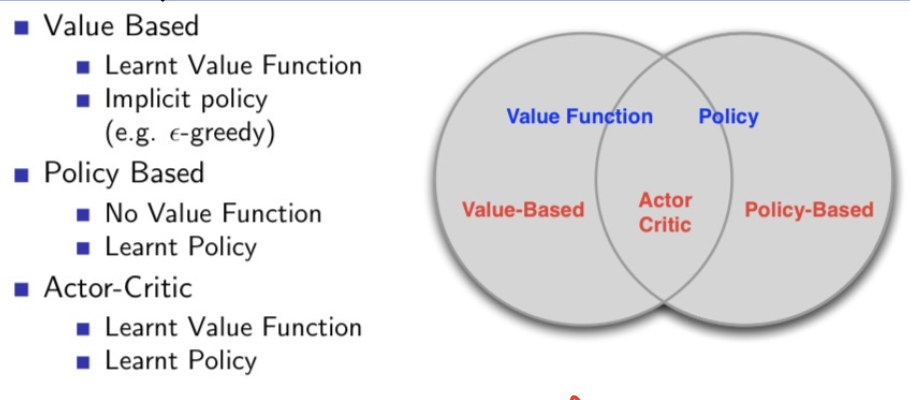
\includegraphics[width=0.5\linewidth]{valuepolicy.png}
    \label{fig:enter-label}
\end{figure}
\subsection{Bellman Equation}
The Bellman equation expresses the value of a state as the immediate reward plus the expected discounted value of future states, enabling recursive computation of optimal policies in dynamic programming. It is written as:

\[
V(s) = \max_a \left[ R(s, a) + \gamma \sum_{s'} P(s' | s, a) V(s') \right]
\]

where \( V(s) \) is the value function, \( R(s, a) \) is the reward, \( \gamma \) is the discount factor, and \( P(s' | s, a) \) is the transition probability.

\subsection{Policy Gradient}
\begin{itemize}
    \item Use sign of reward on gradient. Encourages actions leading to win, discourage others.
    \item Generalizes likelihood ratio approach to multi step MDP
    \item Replaces instanaeous reward r with long-term value Q
\end{itemize}
\subsection{Markov Chain}
Stochastic process where next state depends on current state. Uses \textbf{states, transition probabilities and is memoryless}.
\subsection{Markov Decision Processes (MDPs)}
\begin{itemize}
    \item Defined by states $S$, actions $A$, transition probabilities $P(s'|s, a)$, and rewards $R(s, a)$.
    \item Markov property: Future state depends only on the current state and action.
    \item Bellman equation for state-value function:
    \[ V(s) = \mathbb{E}_{a \sim \pi}[R(s, a) + \gamma V(s')]. \]
    \item Deep Q-Learning is algorithn to solve MDPs and approximates $Q(s, a)$ using a neural network and minimizes:
    \[ \mathcal{L}(\theta) = \mathbb{E}[(Q(s, a; \theta) - y)^2], \]
    where $y = r + \gamma \max_{a'} Q(s', a'; \theta').$
\end{itemize}

\subsection{Hidden Markov Models (HMMs)}
\begin{itemize}
    \item Represents processes with hidden states $Z$ and observations $X$.
    \item Components:
    \begin{itemize}
        \item Initial state probabilities $P(z_1)$.
        \item Transition probabilities $P(z_{t+1}|z_t)$.
        \item Emission probabilities $P(x_t|z_t)$, represent the probability of observing a particular output (or emission $x_t$) given a hidden state.
    \end{itemize}
    \item Forward algorithm computes observation likelihood:
    \[ \alpha_t(z) = \sum_{z'} \alpha_{t-1}(z') P(z|z') P(x_t|z). \]
    $\alpha_t(z)$ is the probability of observing the first  $t$ observations and ending up in state $z$
\end{itemize}

\subsection{Monte Carlo Methods:}
    \begin{itemize}
    \item Monte Carlo methods estimate values by running many random simulations and averaging the results, making them useful for solving problems where exact solutions are difficult or infeasible.
        \item Estimate value functions using episodic returns.
        \item Updates policies parameters based on sampled trajectories:
        \[ \theta \leftarrow \theta + \alpha \nabla \log \pi_\theta(a|s) G_t, \]
        where $G_t$ is the return from timestep $t$.
    \end{itemize}
\subsection{Monte Carlo Tree Search (MCTS):} Explores decision trees by simulating play and propagating values up the tree.

\subsection{Multi-Armed Bandits:} Models decision-making with $k$ independent actions (arms):
    \begin{itemize}
        \item \textbf{Epsilon-Greedy:} Chooses random actions with probability $\epsilon$, otherwise exploits the best-known action.
        \item \textbf{Upper Confidence Bound (UCB):} Balances exploration and exploitation based on action uncertainty:
        \[ a_t = \arg\max_a \left( \hat{Q}(a) + c \sqrt{\frac{\log t}{N(a)}} \right), \]
        where $\hat{Q}(a)$ is the estimated reward, $N(a)$ is the number of times action $a$ has been chosen so far, and $c$ controls exploration. Upper Confidence Bound (UCB) is named because it selects actions based on an upper bound on the estimated reward, ensuring that actions with uncertain rewards are explored.
        \item \textbf{Thompson Sampling:} Samples actions proportionally to the probability of being optimal.
    \end{itemize}

\subsection{TD Learning}
\begin{enumerate}
    \item \textbf{Combines Monte Carlo and Dynamic Programming (DP):}
    \begin{itemize}
        \item TD learning estimates value functions by combining ideas from Monte Carlo methods (sampling) and DP (bootstrapping). Bootstrapping refers to the process of updating value estimates using other current estimates rather than relying solely on actual rewards from complete episodes
        \item It updates estimates based on sampled experience and partial future estimates.
    \end{itemize}

    \item \textbf{Incremental Updates:}
    \begin{itemize}
        \item Updates are made after every step rather than waiting until the end of an episode, enabling real-time learning.
        \item The update rule is given by:
        \[
        V(s) \gets V(s) + \alpha \big[ R_{t+1} + \gamma V(s') - V(s) \big]
        \]
        where:
        \begin{itemize}
            \item \( \alpha \): Learning rate.
            \item \( \gamma \): Discount factor.
            \item \( R_{t+1} \): Reward received after the transition.
            \item \( V(s) \): Current estimate of the value of state \( s \).
            \item \( V(s') \): Current estimate of the value of the next state \( s' \).
        \end{itemize}
    \end{itemize}

    \item \textbf{Bootstrapping:}
    \begin{itemize}
        \item TD learning uses the current estimate of the value of the next state (\( V(s') \)) to improve the current estimate (\( V(s) \)).
        \item This is more efficient than waiting for the final outcome of an episode.
    \end{itemize}

    \item \textbf{Key Algorithms:}
    \begin{itemize}
        \item TD learning includes important algorithms such as:
        \begin{itemize}
            \item \textbf{TD(0)}: One-step TD learning.
            \item \textbf{SARSA}: On-policy TD control.
            \item \textbf{Q-learning}: Off-policy TD control.
        \end{itemize}
        \item These algorithms are widely used in reinforcement learning tasks.
    \end{itemize}
\end{enumerate}
\subsection{SARSA:} On-policy algorithm that updates Q-values based on the current policy:
    \[ Q(s, a) \leftarrow Q(s, a) + \alpha \left[ r + \gamma Q(s', a') - Q(s, a) \right]. \]
\subsection{Reinforce}%TODO add details 
\begin{enumerate}
    \item \textbf{Policy Gradient Method:}
    \begin{itemize}
        \item REINFORCE is a Monte Carlo policy gradient algorithm used to optimize a stochastic policy by directly adjusting its parameters.
        \item It maximizes the expected cumulative reward \( J(\theta) \) by following the gradient of the objective:
        \[
        \nabla_\theta J(\theta) = \mathbb{E} \big[ \nabla_\theta \log \pi_\theta(a | s) G_t \big],
        \]
        where \( \pi_\theta(a | s) \) is the policy, and \( G_t \) is the cumulative reward from time \( t \).

    \end{itemize}

    \item \textbf{Monte Carlo Sampling:}
    \begin{itemize}
        \item The algorithm uses sampled trajectories to estimate the gradient without relying on a value function.
        \item Rewards are collected from full episodes, making it suitable for episodic tasks.
    \end{itemize}

    \item \textbf{Updates Based on Rewards:}
    \begin{itemize}
        \item The policy is updated to increase the probability of actions that lead to higher rewards.
        \item The update rule for the policy parameters is:
        \[
        \theta \gets \theta + \alpha \nabla_\theta \log \pi_\theta(a | s) G_t,
        \]
        where \( \alpha \) is the learning rate.
    \end{itemize}

    \item \textbf{Key Characteristics:}
    \begin{itemize}
        \item \textbf{Variance}: The method can have high variance due to its reliance on full-episode returns.
        \item \textbf{Baseline}: Adding a baseline (e.g., value function) can reduce variance without introducing bias. Introducing a \textbf{baseline} \( b(s) \), typically the state value function \( V(s) \), modifies the update:

\[
\theta \leftarrow \theta + \alpha \nabla_{\theta} \log \pi_{\theta}(a | s) (G_t - b(s))
\]

Since \( G_t - b(s) \) centers the updates around zero, it reduces variance without changing the expected value of the gradient.

        \item It is widely used in reinforcement learning tasks with discrete action spaces.
    \end{itemize}
\end{enumerate}
\subsection{Q-Learning:} Off-policy algorithm that learns the optimal policy by maximizing future rewards. The Q-value is updated using the Bellman equation:
        \[
        Q(s, a) \gets Q(s, a) + \alpha \big[ R + \gamma \max_a Q(s', a) - Q(s, a) \big],
        \]
        where:
        \begin{itemize}
            \item \( \alpha \): Learning rate.
            \item \( \gamma \): Discount factor.
            \item \( R \): Immediate reward.
            \item \( s' \): Next state.
        \end{itemize}
\subsection{Deep Q-Learning}
\begin{enumerate}
    \item \textbf{Combines Q-Learning with Deep Neural Networks:}
    \begin{itemize}
        \item Deep Q-Learning extends traditional Q-learning by using a deep neural network (DNN) to approximate the Q-value function \( Q(s, a) \), which predicts the expected cumulative reward for taking action \( a \) in state \( s \).
        \item This approach is effective in handling high-dimensional state spaces, such as images.
    \end{itemize}

    \item \textbf{Q-Value Update Rule:}
    \begin{itemize}
        \item In DQL, the neural network approximates \( Q(s, a) \) and is updated based on the temporal difference error.
    \end{itemize}

    \item \textbf{Experience Replay:}
    \begin{itemize}
        \item A replay buffer stores past experiences \((s, a, R, s')\), which are sampled randomly to train the neural network.
        \item This reduces correlation between training samples and improves learning stability.
    \end{itemize}

    \item \textbf{Target Network for Stability:}
    \begin{itemize}
        \item A separate target network is used to compute the target Q-values, which are periodically updated to match the primary network.
        \item This mitigates instability and divergence during training by preventing the same network from bootstrapping off unstable predictions.
    \end{itemize}
\end{enumerate}

\subsection{Actor-Critic Methods:} 
    \begin{itemize}
        \item Actor updates the policy.
        \item Critic evaluates the action using a value function.
    \end{itemize}
    \begin{enumerate}
    \item \textbf{Combines Policy and Value-Based Methods:}
    \begin{itemize}
        \item Actor-Critic algorithms combine the strengths of policy-based methods (the "Actor") and value-based methods (the "Critic").
        \item The \textbf{Actor} updates the policy \( \pi_\theta(a|s) \) directly to maximize expected rewards.
        \item The \textbf{Critic} estimates the value function \( V_w(s) \) to guide the Actor's updates.
    \end{itemize}

    \item \textbf{Two Neural Networks:}
    \begin{itemize}
        \item The \textbf{Actor Network} outputs the policy (a probability distribution over actions).
        \item The \textbf{Critic Network} predicts the value function (e.g., \( V(s) \) or \( Q(s, a) \)).
    \end{itemize}

    \item \textbf{Policy Gradient Update:}
    \begin{itemize}
        \item The Actor is updated using the policy gradient:
        \[
        \nabla_\theta J(\theta) = \mathbb{E} \big[ \nabla_\theta \log \pi_\theta(a|s) A(s, a) \big],
        \]
        where \( A(s, a) \) is the advantage function, which can be defined as:
        \[
        A(s, a) = Q(s, a) - V(s),
        \]
        or an approximation of the temporal difference error.
    \end{itemize}
\end{enumerate}
\subsection{Advantage Actor Critic}
    \begin{itemize}
    \item \textbf{Combines Policy and Value-Based Methods} – Uses an \textit{actor} (policy \( \pi(a|s) \)) to choose actions and a \textit{critic} (value function \( V(s) \)) to estimate how good a state is, improving learning stability.
    
    \item \textbf{Uses Advantage Function} – Instead of the full return, it computes the \textit{advantage}:
    \[
    A(s, a) = Q(s, a) - V(s)
    \]
    to reduce variance, guiding updates based on how much better an action is than expected.

    \item \textbf{More Sample Efficient} – The critic reduces variance in policy updates, allowing faster and more stable learning compared to pure policy gradient methods like REINFORCE.
    
    \item \textbf{Supports Parallel Training} – A3C (Asynchronous Advantage Actor-Critic) enables multiple agents to explore simultaneously, improving training speed and robustness.
\end{itemize}

\subsection{AlphaGo}
\begin{itemize}
    \item Uses two neural networks:
    \begin{itemize}
        \item Policy network selects actions.
        \item Value network predicts the winner of a given state.
    \end{itemize}
    \item Trains by self-play and reinforcement learning.
    \item Monte Carlo simulations explore possible moves and refine strategies.
\end{itemize}
\subsection{Proximal Policy Optimization (PPO)}
\begin{itemize}
    \item Enhances policy gradient methods by ensuring stable learning.
    \item Clipping restricts the extent of policy changes:
    \[ \mathcal{L}(\theta) = \mathbb{E}[\min(r_t(\theta)A_t, \text{clip}(r_t(\theta), 1 - \epsilon, 1 + \epsilon)A_t)], \]
    where $r_t(\theta)$ is the probability ratio and $A_t$ is the advantage function.
    \item Balances exploration and exploitation effectively.
\end{itemize}

\subsection{Trust Region Policy Optimization (TRPO)}
\begin{itemize}
    \item Ensures stable updates to the policy by enforcing a constraint on the change in the policy distribution.
    \item Uses the KL-divergence as a constraint:
    \[ \mathbb{E}[\text{KL}[\pi_\text{old}(a|s) \| \pi_\text{new}(a|s)]] \leq \delta, \]
    where $\delta$ is a small positive constant.
    \item Optimizes the surrogate objective:
    \[ \mathcal{L}(\theta) = \mathbb{E}\left[\frac{\pi_\text{new}(a|s)}{\pi_\text{old}(a|s)} A(s, a)\right]. \]
\end{itemize}
\subsection{RLHF}
\begin{itemize}
    \item Intergrate human feedback into RL 
    \item Reward Modelling: $r_{\theta}(x,y)$ given prompts $x$ and answers $y_w$ and $y_l$ (preferred and less preferred) 
    \item It minimizes $\mathcal{L}= -\text{log}(r_{\theta}(x,y_w)-r_{\theta}(x,y_l))$
    \item Policy Optimization: Model generates response given prompt. Objective is expected reward from reward model while having similarity to initial fine tuned model.
\end{itemize}
\pagebreak


\end{document}
